








\def\alcoves{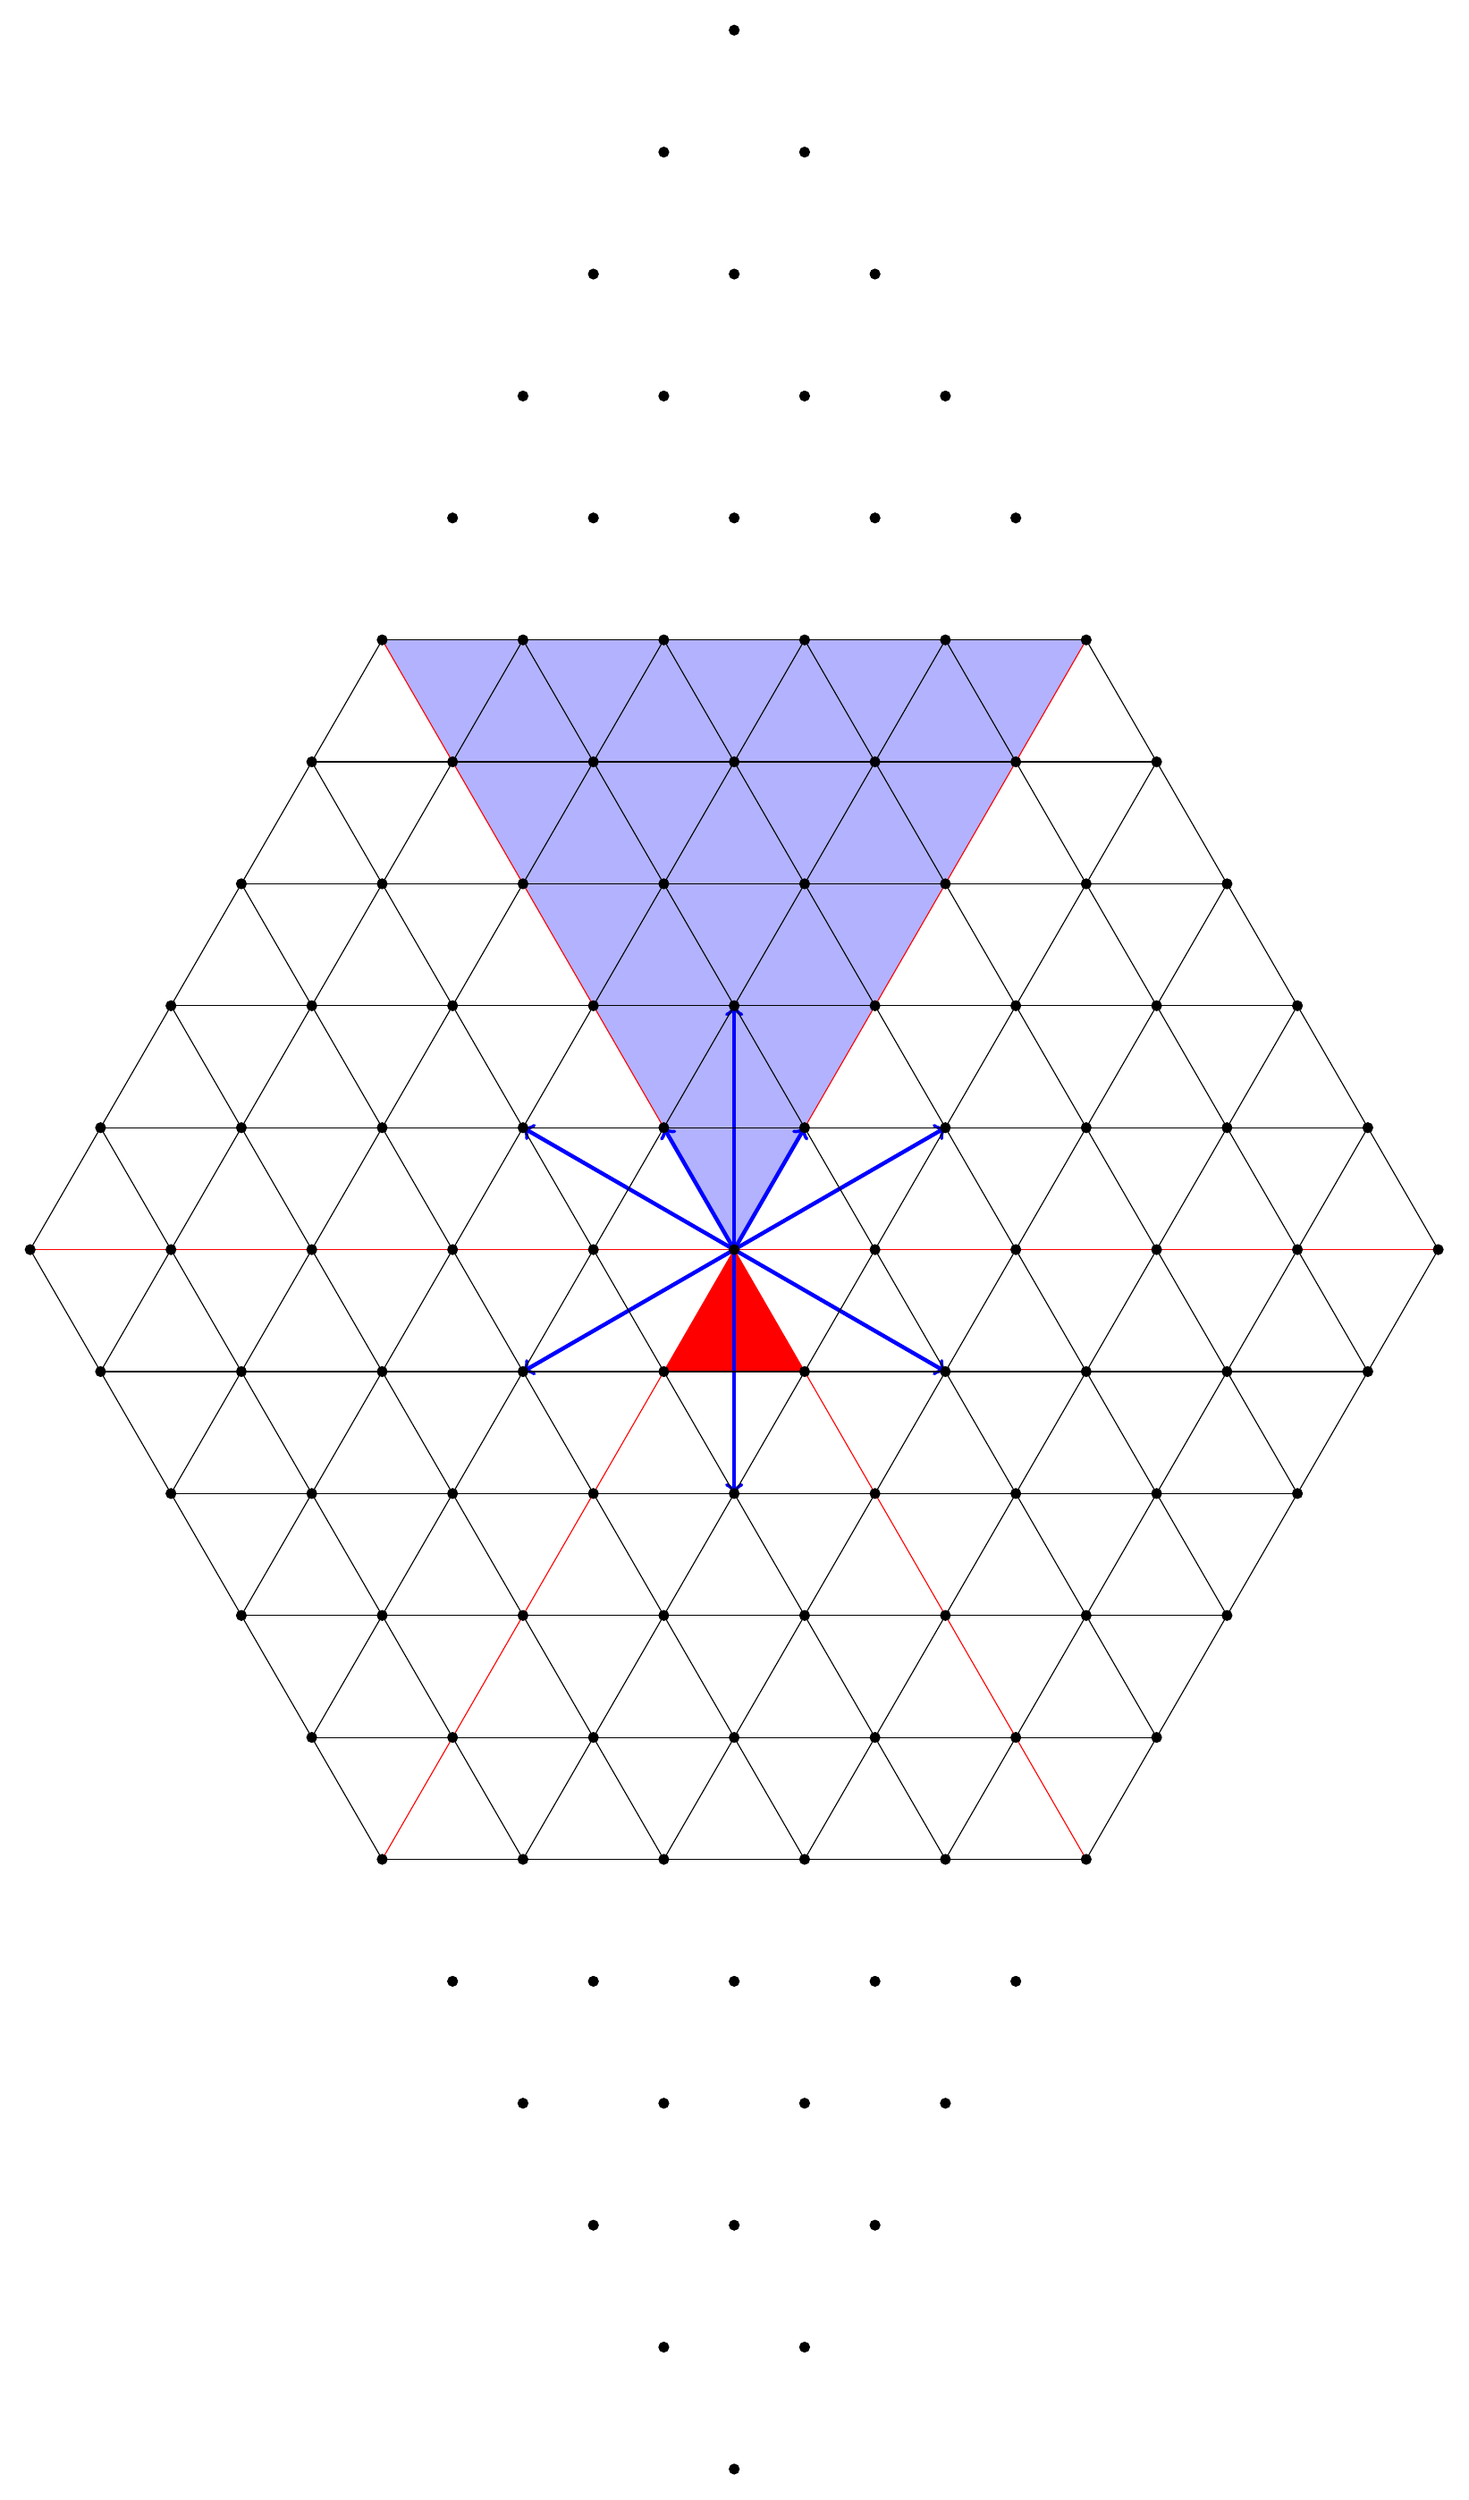
\begin{tikzpicture}
    \fill[blue!30] (0,0) -- (60:10 ) -- (120:10 ) -- cycle;
    \fill[red] (0,0) -- (240:2 ) -- (300:2 ) -- cycle;
    \foreach \i in {0, 1, ..., 5} {
      %\draw[thick, blue] (0, 0) -- (\i*60:2);
      \draw[->, ultra thick, blue] (0, 0) -- (30 + \i*60:3.4641);
      }
      
      % \node[above] at (30:3.4641) {$\alpha_{2}$};
      % \node[above] at (30+1*60:3.4641) {$\alpha_{1}+\alpha_{2}$};
      % \node[above] at (30+2*60:3.4641) {$\alpha_{1}$};
      % \node[below] at (30+3*60:3.4641) {$-\alpha_{2}$};
      % \node[below] at (30+4*60:3.4641) {$-\alpha_{1}-\alpha_{2}$};
      % \node[below] at (30+5*60:3.4641) {$-\alpha_{1}$};
      % \node[above] at (1*60:2) {$\varpi_{1}$};
      % \node[above] at (2*60:2) {$\varpi_{2}$};

    \foreach \m in {0,1,2,3,4,5} {
       \draw[red] (0,0) -- (\m*60:10);
    }
    
      \draw[->, ultra thick, blue] (0, 0) -- (1*60:2);
      \draw[->, ultra thick, blue] (0, 0) -- (2*60:2);
      
      \pgfmathsetmacro\cx{2 * cos(120)}
      \pgfmathsetmacro\sx{2 * sin(120)}
      \pgfmathsetmacro\sy{2 * sin(60)}
      \pgfmathsetmacro\cy{2 * cos(60)}

      \foreach \k in {-5,...,5} {
        \foreach \j in {-5,...,5} {
            %\filldraw (\k*\cx+\j*\cy,\k*\sx+\j*\sy) circle (1.5pt);
            \pgfmathsetmacro\g{\k+\j};
            \ifthenelse{ 6 > \g \AND  -6 < \g  }{\filldraw (\k*\cx+\j*\cy,\k*\sx+\j*\sy) circle (2pt);}{}
        } 
      }
    \foreach \m / \n in {2/8,4/6,6/4,8/2,10/0} {
        \foreach \r in {0,1,2,3,4,5} {
            \draw[shorten >=-\n cm,shorten <=-\n cm] (\r*60 - 60:\m) -- (\r*60:\m);
        }
    }
    %\draw[shorten >=-4cm,shorten <=-4cm] (60:2) -- (120:2);

\end{tikzpicture}}

\def\young{\scalebox{.5}{\ytableausetup{centertableaux}\ydiagram{3,4,5,1,2,4} }. 
}

\def\lambdayoung{\scalebox{.5}{\ytableausetup{centertableaux}\ydiagram{5,4,3,3,3,3,3,3,2,1} }
}

\def\plambdayoung{\scalebox{.5}{\ytableaushort
{\none,\none , \none }
* {5,3,3,3,3,3,3,4,2,1}
* [*(red)]{0,3+1,0}
* [*(green)]{0,0,0,0,0,0,0,3+1}    } 
}

\def\qlambdayoung{\scalebox{.5}{\ytableaushort
{\none,\none , \none }
* {5,4,3,3,3,3,3,3,3,1}
* [*(red)]{0,0,0,0,0,0,0,2+1}
* [*(green)]{0,0,0,0,0,0,0,0,2+1}    }
}

\def\topyounguno{\ytableausetup{centertableaux}\ydiagram{7,6,3,2,2,2,2,2,2,1} 
}

\def\topyoungdos{\ytableaushort
{\none,\none , \none }
* {7,6,3,2,2,2,2,2,2,1}
* [*(red)]{0,5+1}
* [*(green)]{0,0,0,0,0,0,0,2+1}   
}

\def\topyoungtres{\ytableaushort
{\none,\none , \none }
* {7,5,3,2,2,2,2,3,2,1}
* [*(red)]{0,0,2+1}
* [*(green)]{0,0,0,0,0,0,2+1}  
}

\def\topyoungcuatro{\ytableaushort
{\none,\none , \none }
* {7,5,2,2,2,2,3,3,2,1}
* [*(red)]{0,4+1}
* [*(green)]{0,0,0,0,0,2+1} 
}

\def\topyoungcinco{\ytableaushort
{\none,\none , \none }
* {7,4,2,2,2,3,3,3,2,1}
* [*(red)]{6+1}
* [*(green)]{0,0,0,0,2+1}   
}

\def\topyoungseis{\ytableaushort
{\none,\none , \none }
* {6,4,2,2,3,3,3,3,2,1}
* [*(red)]{0,3+1}
* [*(green)]{0,0,0,2+1} 
}

\def\topyoungsiete{\ytableaushort
{\none,\none , \none }
* {6,3,2,3,3,3,3,3,2,1}
* [*(red)]{5+1}
* [*(green)]{0,0,2+1}
}

\def\topyoung{\ytableaushort
{\none,\none , \none }
* {5,3,3,3,3,3,3,3,2,1}
}

\def\belowyounguno{\ytableaushort
{\none,\none , \none }
* {5,3,3,3,3,3,3,3,2,1}
* [*(red)]{0,0,0,0,0,0,0,2+1}
* [*(green)]{0,0,0,0,0,0,0,0,0,1+1}
}

\def\caseuno{
\begin{tikzpicture}
\draw[red] (0,1) -- (5,1);
\draw (2.5,1) -- (2.5,0) -- (3.5,0) -- (3.5,1);
\draw (3,0.5) node {\huge s};
\draw (2.5,0) -- (2.5,-2);
\draw[red] (0,-2) -- (5,-2);
\draw (1.5,-2) -- (1.5,-3) -- (2.5,-3) -- (2.5,-2);
\draw (2,-2.5) node {\huge t};
\draw[red] (0,-5) -- (5,-5);
\draw[->, red] (2,-4) -- (2,-3);
\draw (1.5,-5) -- (1.5,-4) -- (2.5,-4) -- (2.5,-5);
\draw (2,-4.5) node {\huge r};
\draw (0,1) -- (0,-5);
\end{tikzpicture}
}

\def\casedos{
\begin{tikzpicture}
\draw[red] (0,1) -- (5,1);
\draw (2.5,1) -- (2.5,0) -- (3.5,0) -- (3.5,1);
\draw (1.5,1) -- (1.5,0)-- (2.5,0);
\draw (3,0.5) node {\huge t};
\draw (2,0.5) node {\huge s};
\draw[->, red] (2,-1) -- (2,-0.1);
\draw[red] (0,-2) -- (5,-2);
\draw (1.5,-2) -- (1.5,-1) -- (2.5,-1) --  (2.5,-2);
\draw (2,-1.5) node {\huge r};
\end{tikzpicture}
}

\def\casetres{
\begin{tikzpicture}
\draw[red] (0,1) -- (5,1);
\draw (2.5,1) -- (2.5,0) -- (3.5,0) -- (3.5,1);
\draw (3,0.5) node {\huge s};
\draw (1.5,-2) -- (1.5,-1)  -- (2.5,-1) --  (2.5,-2);
\draw (2,-1.5) node {\huge r};
\draw[red] (0,-2) -- (5,-2);
\draw (1.5,-2) -- (1.5,-3)  -- (2.5,-3) --  (2.5,-2);
\draw (2,-2.5) node {\huge t};
\draw[->, rounded corners=12pt, red ] (2,-1) -- (2,-0.5) -- (4,-0.5) -- (4,-4) -- (2,-4) -- (2,-3);
\draw[red] (0,-5) -- (5,-5);
\end{tikzpicture}
}

\def\casecuatro{
\begin{tikzpicture}
\draw[red] (0,1) -- (5,1);
\draw (2.5,1) -- (2.5,0) -- (3.5,0) -- (3.5,1);
\draw (3,0.5) node {\huge s};
\draw[red] (0,-2) -- (5,-2);
\draw (1.5,-2) -- (1.5,-3) -- (2.5,-3) -- (2.5,-2);
\draw (2,-2.5) node {\huge t};
\draw[red] (0,-5) -- (5,-5);
\draw[->, red] (2,-4) -- (2,-3);
\draw (1.5,-5) -- (1.5,-4) -- (2.5,-4) -- (2.5,-5);
\draw (2,-4.5) node {\huge r};
\end{tikzpicture}
}

\def\exacaseunouno{
\begin{equation}
\scalebox{.5}{ \ytableausetup{centertableaux}
\ytableaushort
{\none, \none , \none }
* {7,5,5,5,5,4,3,3,3,3,2,1}}
\xrightarrow{B_{i,j}}
\scalebox{.5}{\ytableausetup{centertableaux}
\ytableaushort
{\none, \none , \none }
* {7,5,5,5,5,4,3,3,3,3,2,1} 
* [*(red) ] {6+1}
* [*(green) ] {0,0,0,0,0,0,0,0,0,0,0,1+1}}
\xrightarrow{P_{6,8}}
\scalebox{.5}{\ytableausetup{centertableaux}
\ytableaushort
{\none, \none , \none }
* {6,5,5,5,5,4,3,3,3,3,2,2} 
* [*(red) ] {0,0,0,0,0,3+1}
* [*(green) ] {0,0,0,0,0,0,0,0,3+1}}
\xrightarrow{P_{5,7}}
\scalebox{.5}{\ytableausetup{centertableaux}
\ytableaushort
{\none, \none , \none }
* {6,5,5,5,5,3,3,3,4,3,2,2} 
* [*(red) ] {0,0,0,0,4+1}
* [*(green) ] {0,0,0,0,0,0,0,3+1}}
\xrightarrow{P_{4,6}}
\scalebox{.5}{\ytableausetup{centertableaux}
\ytableaushort
{\none, \none , \none }
* {6,5,5,5,4,3,3,4,4,3,2,2} 
* [*(red) ] {0,0,0,4+1}
* [*(green) ] {0,0,0,0,0,0,3+1}}
\xrightarrow{P_{7,9}}
\scalebox{.5}{\ytableausetup{centertableaux}
\ytableaushort
{\none, \none , \none }
* {6,5,5,4,4,3,4,4,4,3,2,2} 
* [*(red) ] {5+1}
* [*(green) ] {0,0,0,0,0,0,0,0,0,3+1}}
\end{equation}
}

\def\exacaseunodos{\begin{equation}
\scalebox{.5}{ \ytableausetup{centertableaux}
\ytableaushort
{\none, \none , \none }
* {7,5,5,5,5,4,3,3,3,3,2,1}}
\xrightarrow{B_{7,9}}
\scalebox{.5}{\ytableausetup{centertableaux}
\ytableaushort
{\none, \none , \none }
* {7,5,5,5,5,4,3,3,3,3,2,1} 
* [*(red) ] {6+1}
* [*(green) ] {0,0,0,0,0,0,0,0,0,0,0,1+1}}
\xrightarrow{P_{7,9}}
\scalebox{.5}{\ytableausetup{centertableaux}
\ytableaushort
{\none, \none , \none }
* {6,5,5,5,5,4,3,3,3,3,2,1} 
* [*(red) ] {5+1}
* [*(green) ] {0,0,0,0,0,0,0,0,0,3+1}}
\xrightarrow{P_{6,8}}
\scalebox{.5}{\ytableausetup{centertableaux}
\ytableaushort
{\none, \none , \none }
* {5,5,5,5,5,4,3,3,3,4,2,2} 
* [*(red) ] {0,0,0,0,0,3+1}
* [*(green) ] {0,0,0,0,0,0,0,0,3+1}}
\xrightarrow{P_{5,7}}
\scalebox{.5}{\ytableausetup{centertableaux}
\ytableaushort
{\none, \none , \none }
* {5,5,5,5,5,3,3,3,4,4,2,2} 
* [*(red) ] {0,0,0,0,4+1}
* [*(green) ] {0,0,0,0,0,0,0,3+1}}
\xrightarrow{P_{4,6}}
\scalebox{.5}{\ytableausetup{centertableaux}
\ytableaushort
{\none, \none , \none }
* {5,5,5,5,4,3,3,4,4,4,2,2} 
* [*(red) ] {0,0,0,4+1}
* [*(green) ] {0,0,0,0,0,0,3+1}}
\end{equation}}

\def\exacasedosuno{\begin{equation}
\scalebox{.5}{ \ytableausetup{centertableaux}
\ytableaushort
{\none, \none , \none }
* {5,5,5,4,4,2,2,2,2,2,2,2,1}}
\xrightarrow{B_{8,10}}
\scalebox{.5}{ \ytableausetup{centertableaux}
\ytableaushort
{\none, \none , \none }
* {5,5,5,4,4,2,2,2,2,2,2,2,1}
* [*(red) ] {0,0,0,0,3+1}
* [*(green) ] {0,0,0,0,0,0,0,0,0,0,0,0,1+1}}
\xrightarrow{P_{8,10}}
\scalebox{.5}{ \ytableausetup{centertableaux}
\ytableaushort
{\none, \none , \none }
* {5,5,5,4,3,2,2,2,2,2,2,2,2}
* [*(red) ] {0,0,0,0,2+1}
* [*(green) ] {0,0,0,0,0,0,0,0,0,0,2+1}}
\xrightarrow{P_{7,9}}
\scalebox{.5}{ \ytableausetup{centertableaux}
\ytableaushort
{\none, \none , \none }
* {5,5,5,4,2,2,2,2,2,2,3,2,2}
* [*(red) ] {0,0,0,3+1}
* [*(green) ] {0,0,0,0,0,0,0,0,0,2+1}}
\xrightarrow{P_{6,8}}
\scalebox{.5}{ \ytableausetup{centertableaux}
\ytableaushort
{\none, \none , \none }
* {5,5,5,3,2,2,2,2,2,3,3,2,2}
* [*(red) ] {0,0,4+1}
* [*(green) ] {0,0,0,0,0,0,0,0,2+1}}
\xrightarrow{P_{5,7}}
\scalebox{.5}{ \ytableausetup{centertableaux}
\ytableaushort
{\none, \none , \none }
* {5,5,4,3,2,2,2,2,3,3,3,2,2}
* [*(red) ] {0,4+1}
* [*(green) ] {0,0,0,0,0,0,0,2+1}}
\end{equation}}

\def\exacasedosdos{\begin{equation}
\scalebox{.5}{ \ytableausetup{centertableaux}
\ytableaushort
{\none, \none , \none }
* {5,5,5,4,4,2,2,2,2,2,2,2,1}}
\xrightarrow{B_{8,10}}
\scalebox{.5}{ \ytableausetup{centertableaux}
\ytableaushort
{\none, \none , \none }
* {5,5,5,4,4,2,2,2,2,2,2,2,1}
* [*(red) ] {0,0,0,0,3+1}
* [*(green) ] {0,0,0,0,0,0,0,0,0,0,0,0,1+1}}
\xrightarrow{P_{7,9}}
\scalebox{.5}{ \ytableausetup{centertableaux}
\ytableaushort
{\none, \none , \none }
* {5,5,5,4,3,2,2,2,2,2,2,2,2}
* [*(red) ] {0,0,0,3+1}
* [*(green) ] {0,0,0,0,0,0,0,0,0,2+1}}
\xrightarrow{P_{6,8}}
\scalebox{.5}{ \ytableausetup{centertableaux}
\ytableaushort
{\none, \none , \none }
* {5,5,5,3,3,2,2,2,2,3,2,2,2}
* [*(red) ] {0,0,4+1}
* [*(green) ] {0,0,0,0,0,0,0,0,2+1}}
\xrightarrow{P_{5,7}}
\scalebox{.5}{ \ytableausetup{centertableaux}
\ytableaushort
{\none, \none , \none }
* {5,5,4,3,3,2,2,2,3,3,2,2,2}
* [*(red) ] {0,0,0,0,2+1}
* [*(green) ] {0,0,0,0,0,0,0,2+1}}
\xrightarrow{P_{8,10}}
\scalebox{.5}{ \ytableausetup{centertableaux}
\ytableaushort
{\none, \none , \none }
* {5,5,4,3,2,2,2,3,3,3,2,2,2}
* [*(red) ] {0,4+1}
* [*(green) ] {0,0,0,0,0,0,0,0,0,0,2+1}}
\end{equation}}

\def\exacasetresuno{\begin{equation}
\scalebox{.5}{ \ytableausetup{centertableaux}
\ytableaushort
{\none, \none , \none }
* {5,5,5,4,4,2,2,2,2,2,2,2,1}}
\xrightarrow{\tilde{P}_{0}B_{8,10}}
\scalebox{.5}{ \ytableausetup{centertableaux}
\ytableaushort
{\none, \none , \none }
* {5,5,4,3,2,2,2,3,3,3,2,2,2}}
\xrightarrow{P_{8,10}}
\scalebox{.5}{ \ytableausetup{centertableaux}
\ytableaushort
{\none, \none , \none }
* {5,5,4,3,2,2,2,3,3,3,3,2,2}
* [*(red) ] {0,4+1}
* [*(green) ] {0,0,0,0,0,0,0,0,0,0,2+1}}
\xrightarrow{P_{4,6}}
\scalebox{.5}{ \ytableausetup{centertableaux}
\ytableaushort
{\none, \none , \none }
* {5,4,4,3,2,2,2,3,3,3,3,2,2}
* [*(red) ] {0,0,0,2+1}
* [*(green) ] {0,0,0,0,0,0,2+1}}
\xrightarrow{P_{3,5}}
\scalebox{.5}{ \ytableausetup{centertableaux}
\ytableaushort
{\none, \none , \none }
* {5,4,4,2,2,2,3,3,3,3,3,2,2}
* [*(red) ] {0,0,3+1}
* [*(green) ] {0,0,0,0,0,2+1}}
\xrightarrow{P_{2,4}}
\scalebox{.5}{ \ytableausetup{centertableaux}
\ytableaushort
{\none, \none , \none }
* {5,4,3,2,2,3,3,3,3,3,3,2,2}
* [*(red) ] {0,3+1}
* [*(green) ] {0,0,0,0,2+1}}
\end{equation}
}

\def\exacasetresdos{\begin{equation}
\scalebox{.5}{ \ytableausetup{centertableaux}
\ytableaushort
{\none, \none , \none }
* {5,5,5,4,4,2,2,2,2,2,2,2,1}}
\xrightarrow{\tilde{P}_{0}B_{8,10}}
\scalebox{.5}{ \ytableausetup{centertableaux}
\ytableaushort
{\none, \none , \none }
* {5,5,4,3,2,2,2,3,3,3,2,2,2}}
\xrightarrow{P_{4,6}}
\scalebox{.5}{ \ytableausetup{centertableaux}
\ytableaushort
{\none, \none , \none }
* {5,5,4,3,2,2,2,3,3,3,2,2,2}
* [*(red) ] {0,0,0,2+1}
* [*(green) ] {0,0,0,0,0,0,2+1}}
\xrightarrow{P_{3,5}}
\scalebox{.5}{ \ytableausetup{centertableaux}
\ytableaushort
{\none, \none , \none }
* {5,5,4,2,2,2,3,3,3,3,2,2,2}
* [*(red) ] {0,0,3+1}
* [*(green) ] {0,0,0,0,0,2+1}}
\xrightarrow{P_{2,4}}
\scalebox{.5}{ \ytableausetup{centertableaux}
\ytableaushort
{\none, \none , \none }
* {5,5,3,2,2,3,3,3,3,3,2,2,2}
* [*(red) ] {0,4+1}
* [*(green) ] {0,0,0,0,2+1}}
\xrightarrow{P_{8,10}}
\scalebox{.5}{ \ytableausetup{centertableaux}
\ytableaushort
{\none, \none , \none }
* {5,4,3,2,2,3,3,3,3,3,2,2,2}
* [*(red) ] {0,3+1}
* [*(green) ] {0,0,0,0,0,0,0,0,0,0,2+1}}
\end{equation}
}

\def\positiveroots{
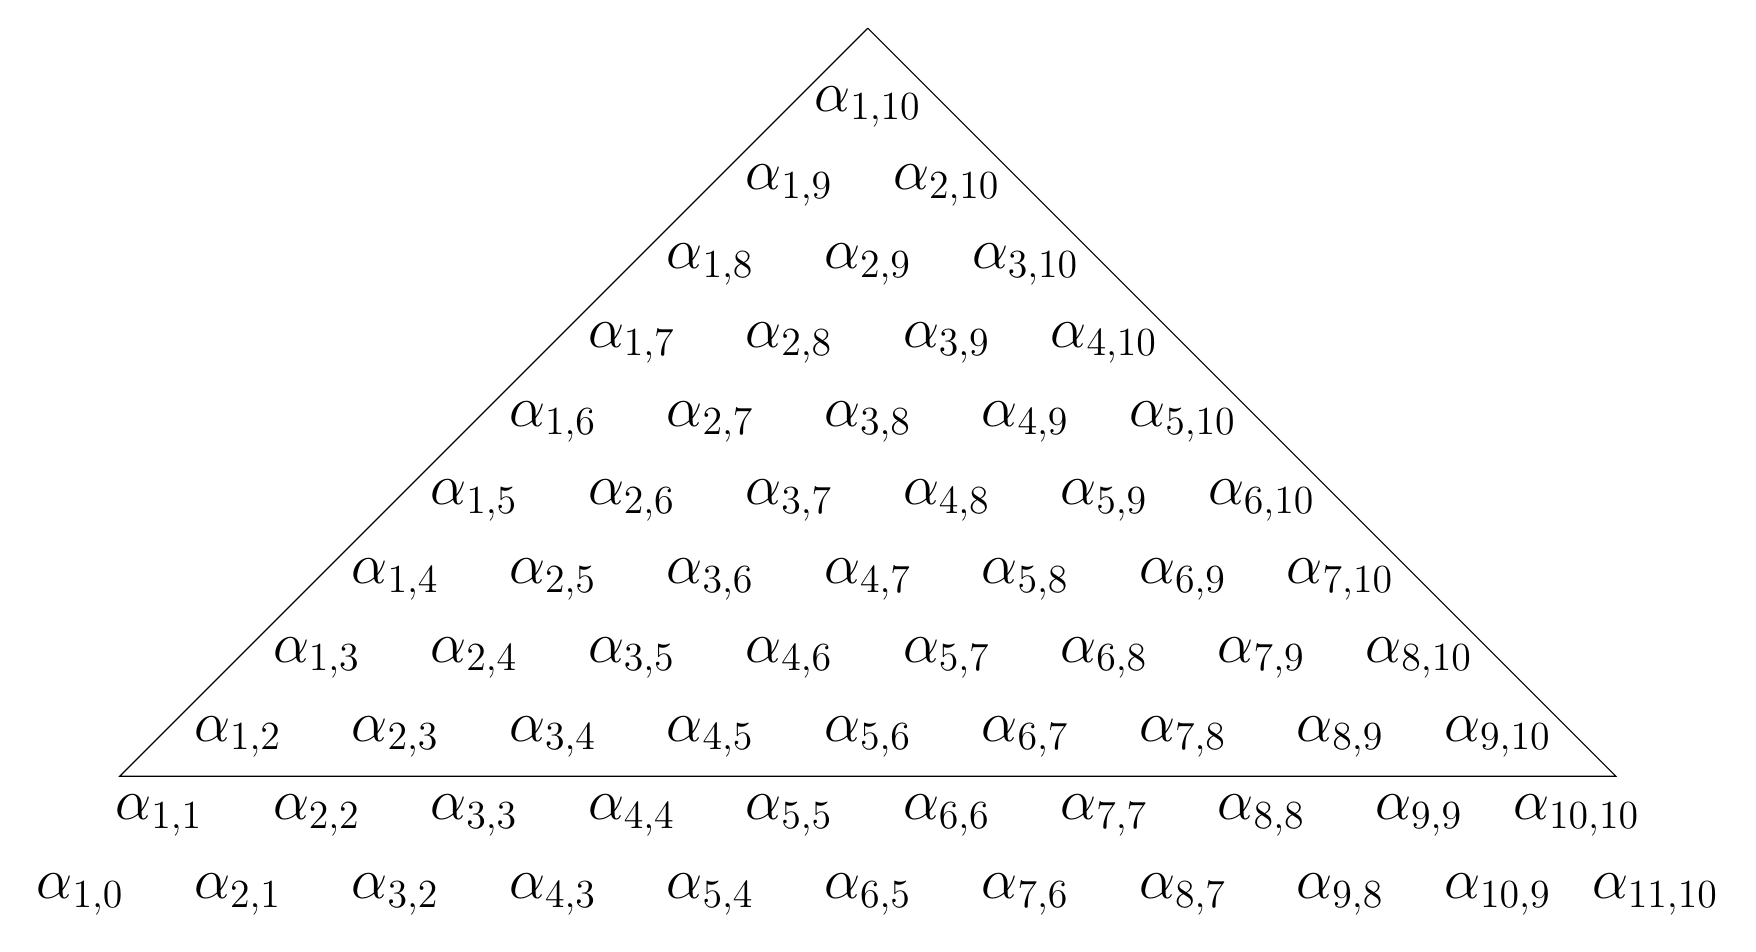
\begin{tikzpicture}[baseline={(-5,-3)}]
\draw (-2,1) -- (-11.5,-8.5) -- (7.5, -8.5) -- (-2,1);
%[fill, green!20!]
\foreach \y in {0,...,10}
    \foreach \x in {0,..., \y }{
        \pgfmathsetmacro\cx{int(\x + 1)};
        \pgfmathsetmacro\cy{int(10 - \y + \x)};
        \pgfmathsetmacro\z{int(10 - \y - 1)};
        \ifthenelse{ \z > 0 }{ 
        \draw (-\y + 2*\x-2,-\y) node {\huge $\alpha_{\cx,\cy}$};}{}
       }

\end{tikzpicture}
}

\def\positiverootsgeqcincosiete{
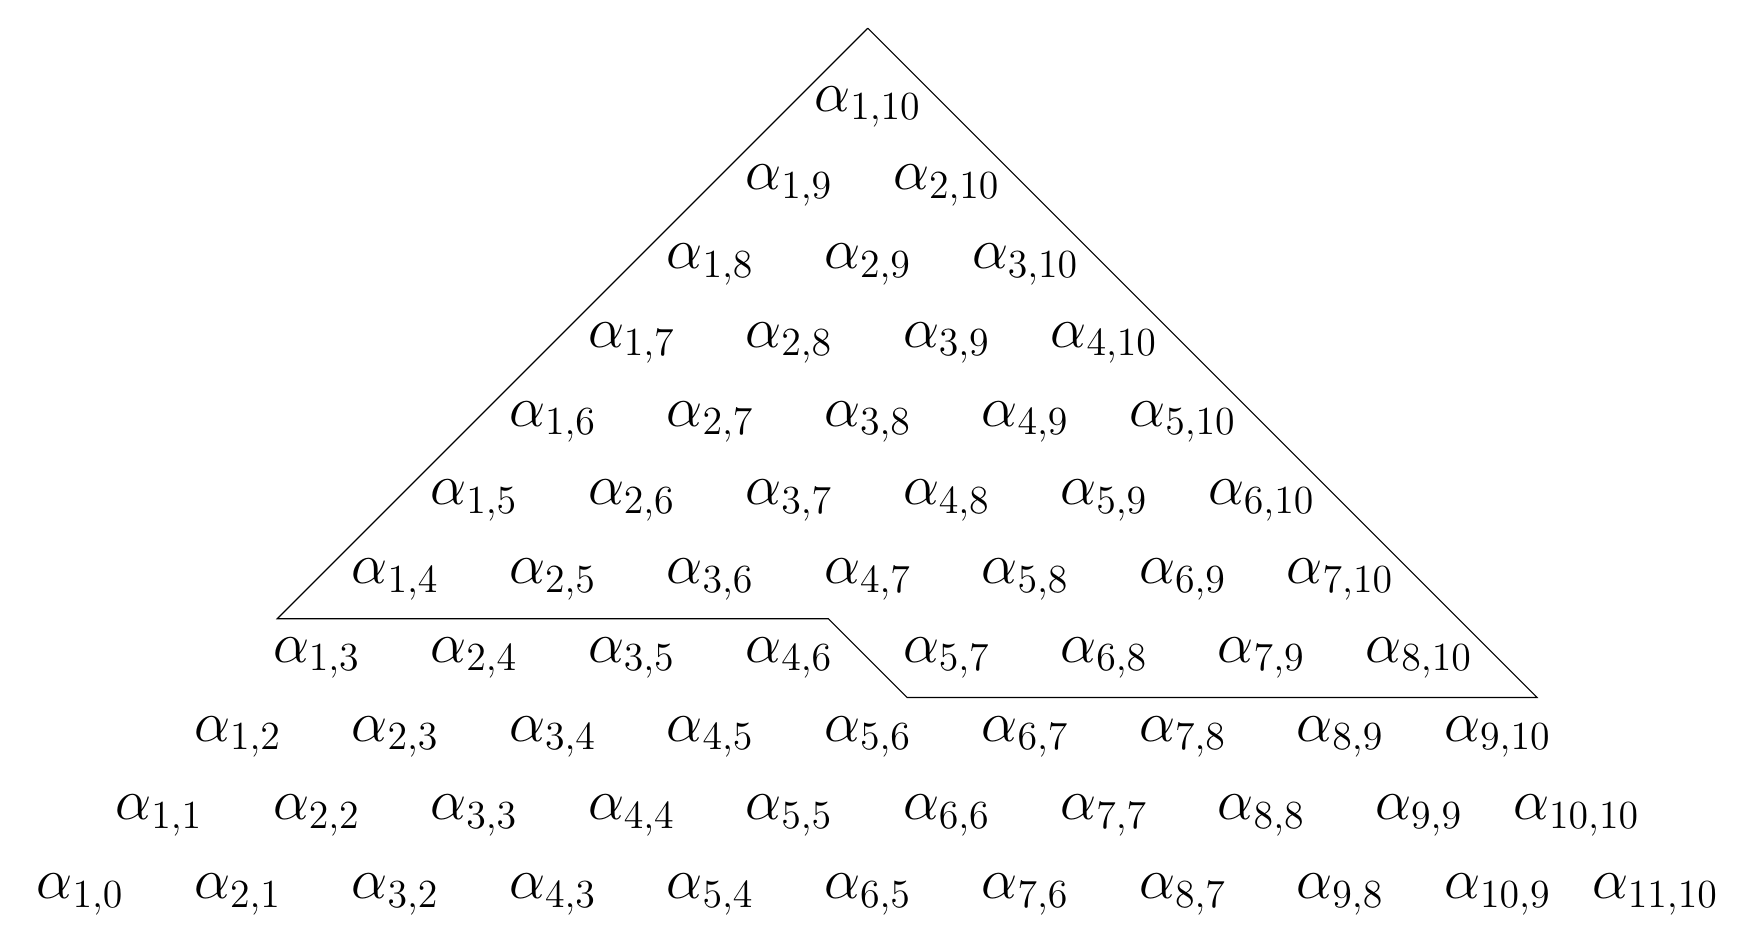
\begin{tikzpicture}[baseline={(-5,-3)}]
\draw (-2,1) -- (-9.5,-6.5) -- (-2.5,-6.5) -- (-1.5,-7.5) -- (6.5, -7.5) -- (-2,1);
%[fill, green!20!]
\foreach \y in {0,...,10}
    \foreach \x in {0,..., \y }{
        \pgfmathsetmacro\cx{int(\x + 1)};
        \pgfmathsetmacro\cy{int(10 - \y + \x)};
        \pgfmathsetmacro\z{int(10 - \y - 1)};
        \ifthenelse{ \z > 1 }{ 
        \draw (-\y + 2*\x-2,-\y) node {\huge $\alpha_{\cx,\cy}$};}{}
       }

\end{tikzpicture}
}

\def\actionofsseisincincosiete{
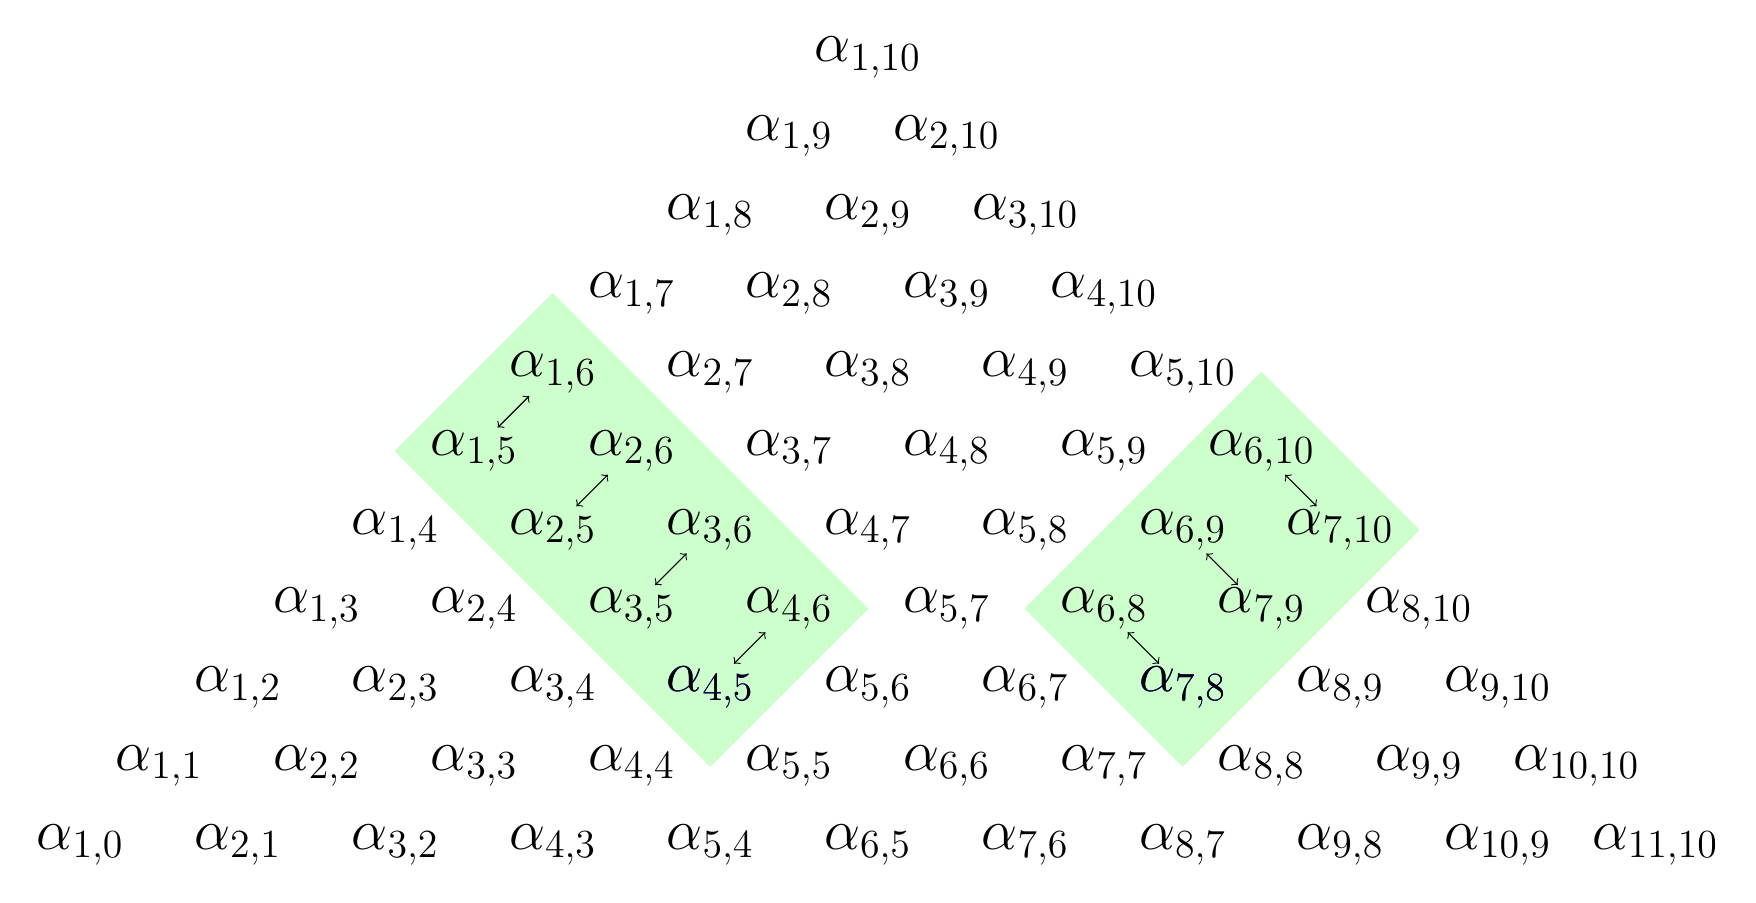
\begin{tikzpicture}[baseline={(-5,-3)}]
%\draw (-2,1) -- (-9.5,-6.5) -- (-2.5,-6.5) -- (-1.5,-7.5) -- (6.5, -7.5) -- (-2,1);
\draw[fill, green!20!] (-8,-5) -- (-6,-3) -- (-2,-7) -- (-4,-9) -- (-8,-5);
\draw[fill, green!20!] (3,-4) -- (5,-6) -- (2,-9) -- (0,-7)-- (3,-4);
\draw[blue] (2,-8) node {\huge $\alpha_{7,8}$};
\draw[blue] (-4,-8) node {\huge $\alpha_{4,5}$};
%[fill, green!20!]

\draw[<->] (-6.3,-4.3) -- (-6.7,-4.7); 
\draw[<->] (-5.3,-5.3) -- (-5.7,-5.7);
\draw[<->] (-4.3,-6.3) -- (-4.7,-6.7);
\draw[<->] (-3.3,-7.3) -- (-3.7,-7.7);

\draw[<->] (3.3,-5.3) -- (3.7,-5.7); 
\draw[<->] (2.3,-6.3) -- (2.7,-6.7);
\draw[<->] (1.3,-7.3) -- (1.7,-7.7);

\foreach \y in {0,...,10}
    \foreach \x in {0,..., \y }{
        \pgfmathsetmacro\cx{int(\x + 1)};
        \pgfmathsetmacro\cy{int(10 - \y + \x)};
        \pgfmathsetmacro\z{int(10 - \y - 1)};
        \ifthenelse{ \z > 1 }{ 
        \draw (-\y + 2*\x-2,-\y) node {\huge $\alpha_{\cx,\cy}$};}{}
       }
\end{tikzpicture}
}

\def\rowfillempty{\ytableausetup{nosmalltableaux}
    \begin{ytableau}
    *(black) & &&&&&  &*(black)  
    \end{ytableau}}

\def\excobkcero{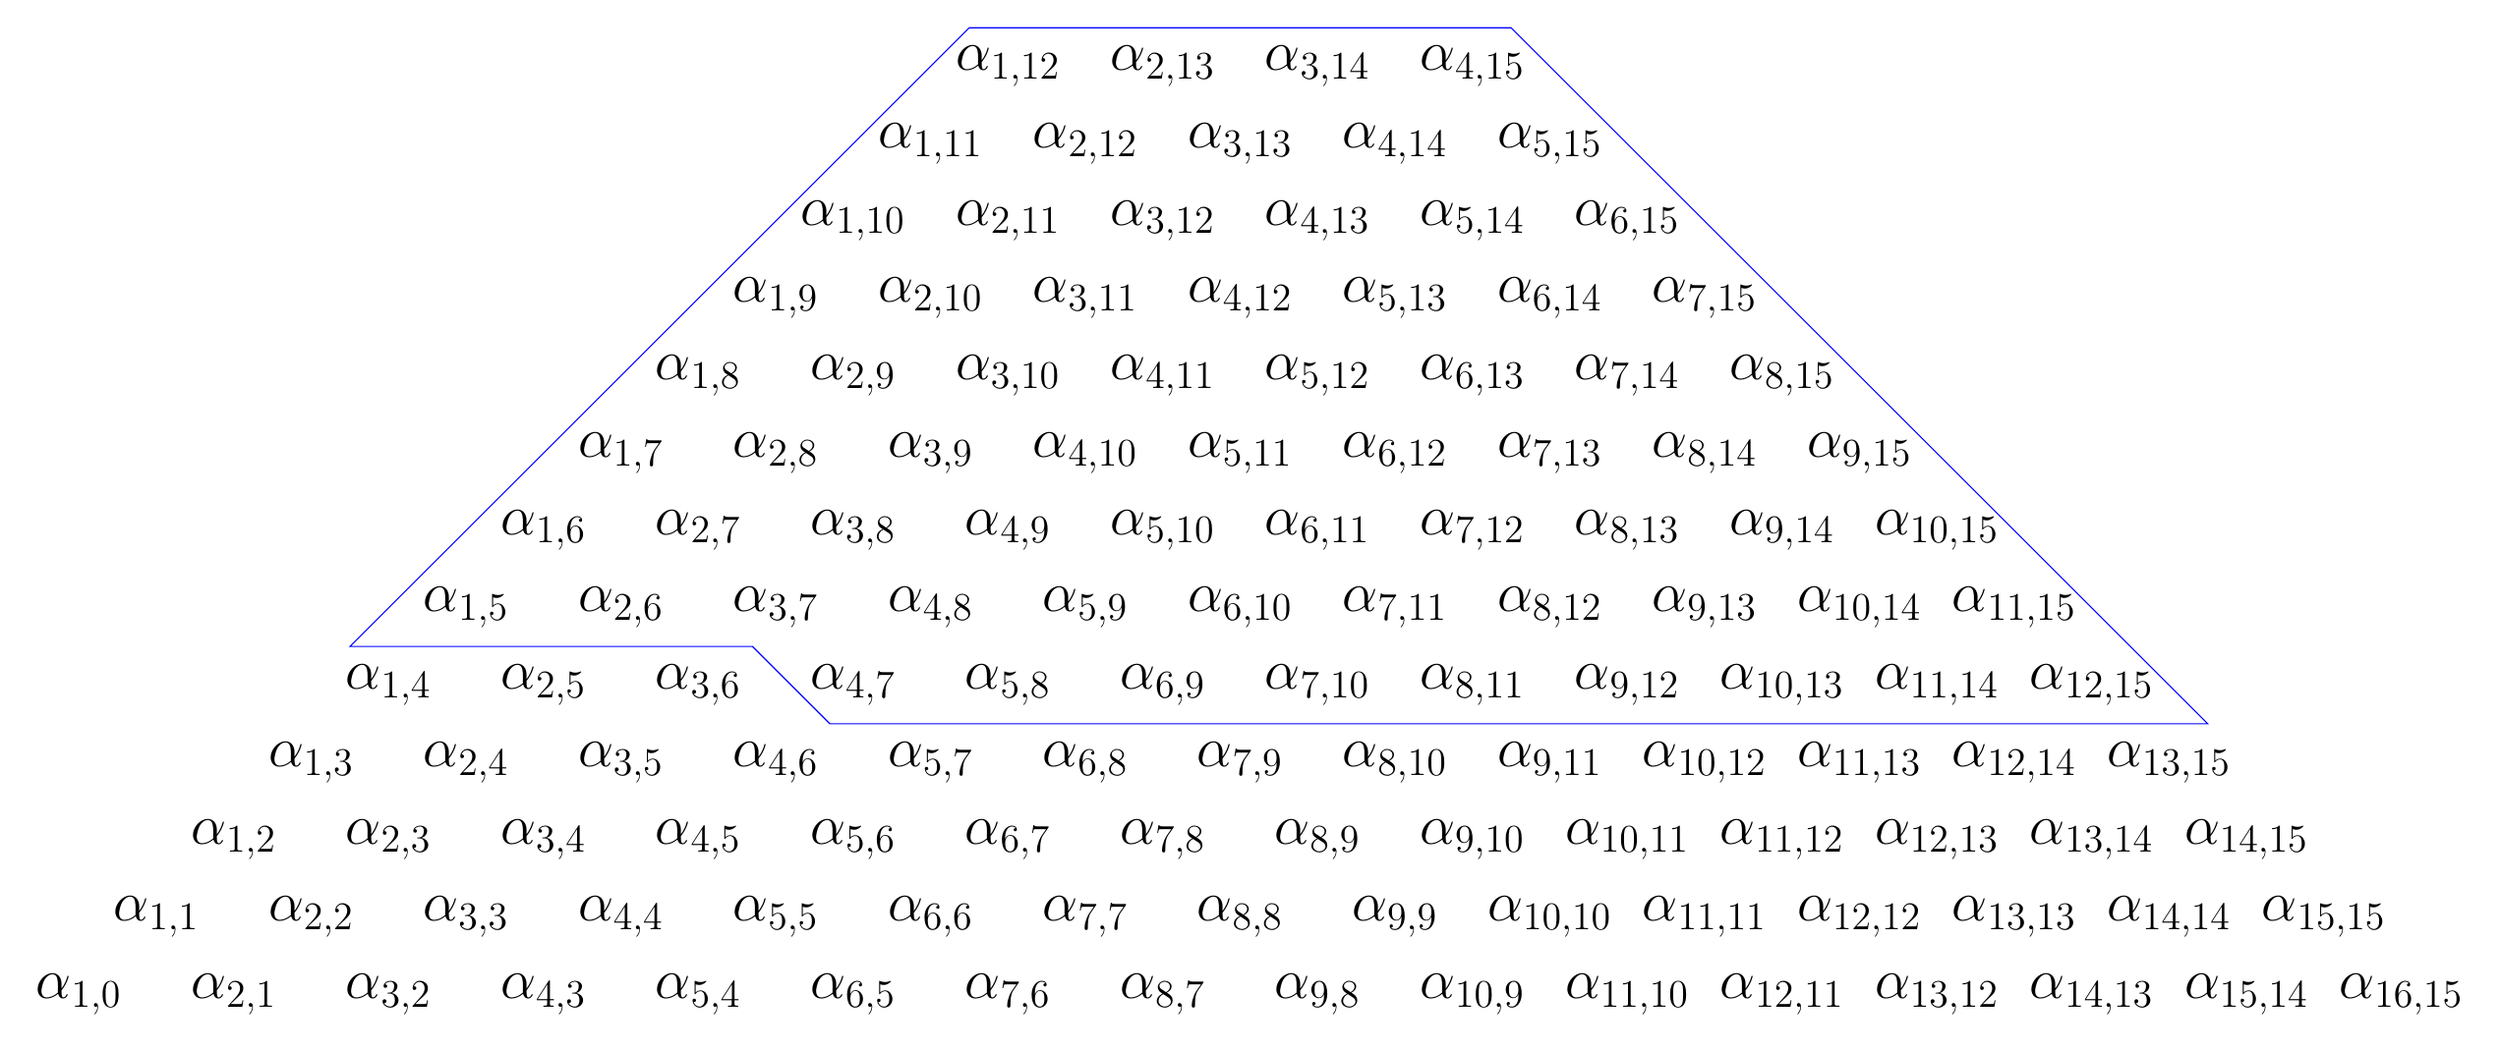
\begin{tikzpicture}[baseline={(0,-7)}]

% \node[draw,fill, red!70!] at (-11,-11) {x  $\alpha_{1,4}$  x};

\foreach \y in {3,...,15}
    \foreach \x in {0,..., \y }{
        \pgfmathsetmacro\cx{int(\x + 1)};
        \pgfmathsetmacro\cy{int(15 - \y + \x)};
        \pgfmathsetmacro\z{int(15 - \y - 1)};
        \ifthenelse{ \z > 2 }{ 
        \draw (-\y + 2*\x ,-\y) node {\huge $\alpha_{\cx,\cy}$};}{}
       }
\draw[blue] (-3.5,-2.5) -- (-11.5,-10.5) -- (-6.3,-10.5) -- (-5.3,-11.5) -- (12.5,-11.5) -- (3.5,-2.5) -- (-3.5,-2.5);

\end{tikzpicture}}

\def\excobkuno{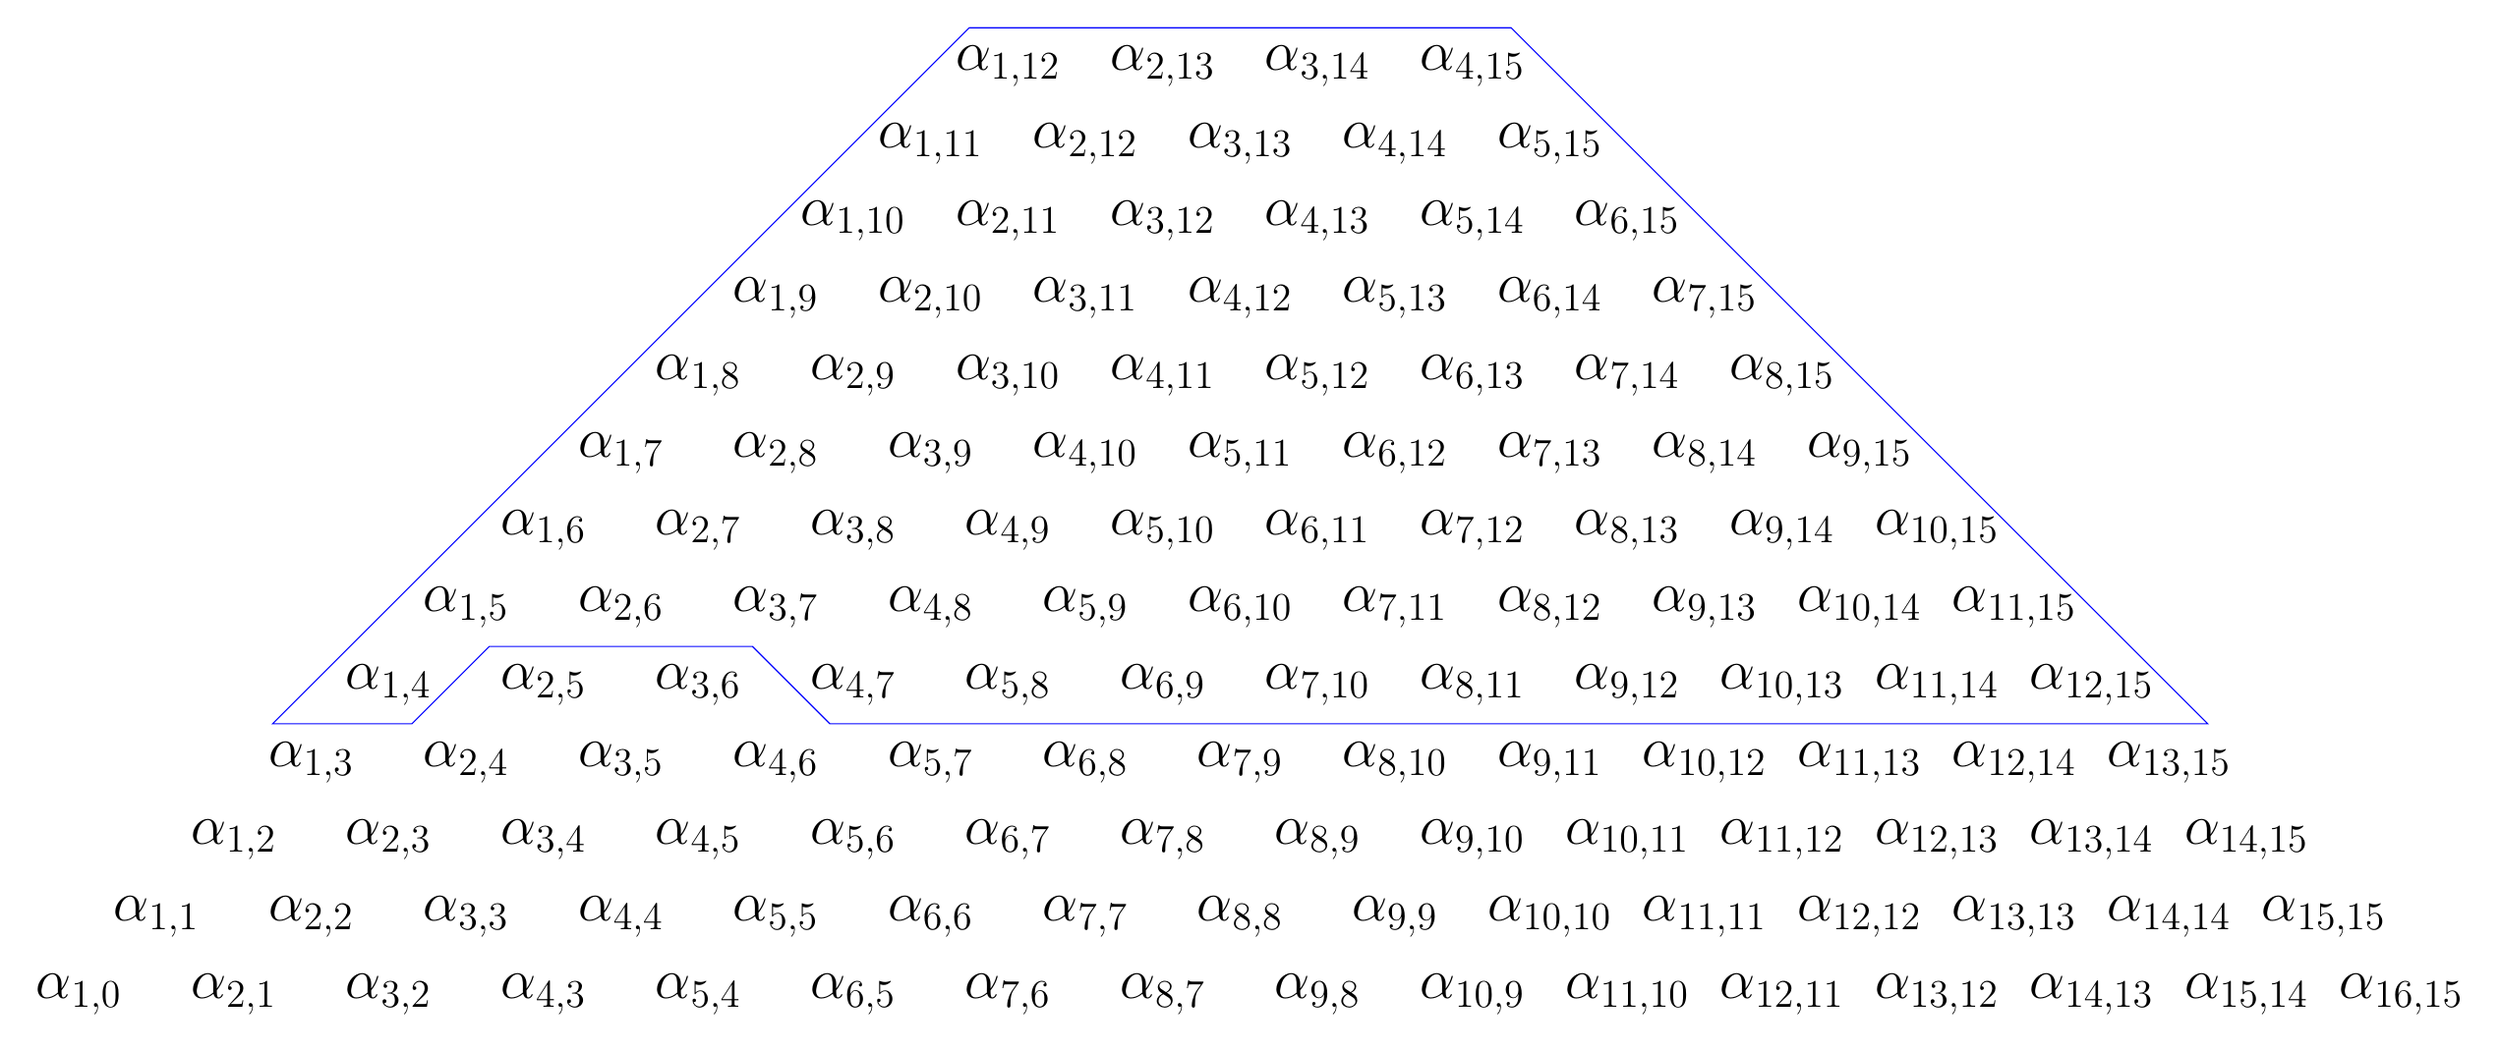
\begin{tikzpicture}[baseline={(0,-7)}]

\foreach \y in {3,...,15}
    \foreach \x in {0,..., \y }{
        \pgfmathsetmacro\cx{int(\x + 1)};
        \pgfmathsetmacro\cy{int(15 - \y + \x)};
        \pgfmathsetmacro\z{int(15 - \y - 1)};
        \ifthenelse{ \z > 2 }{ 
        \draw (-\y + 2*\x ,-\y) node {\huge $\alpha_{\cx,\cy}$};}{}
       }
\draw[blue] (-3.5,-2.5) -- (-12.5,-11.5) -- (-10.7,-11.5) -- (-9.7,-10.5) -- (-6.3,-10.5) -- (-5.3,-11.5) -- (12.5,-11.5) -- (3.5,-2.5) -- (-3.5,-2.5);

\end{tikzpicture}}

\def\excobkdos{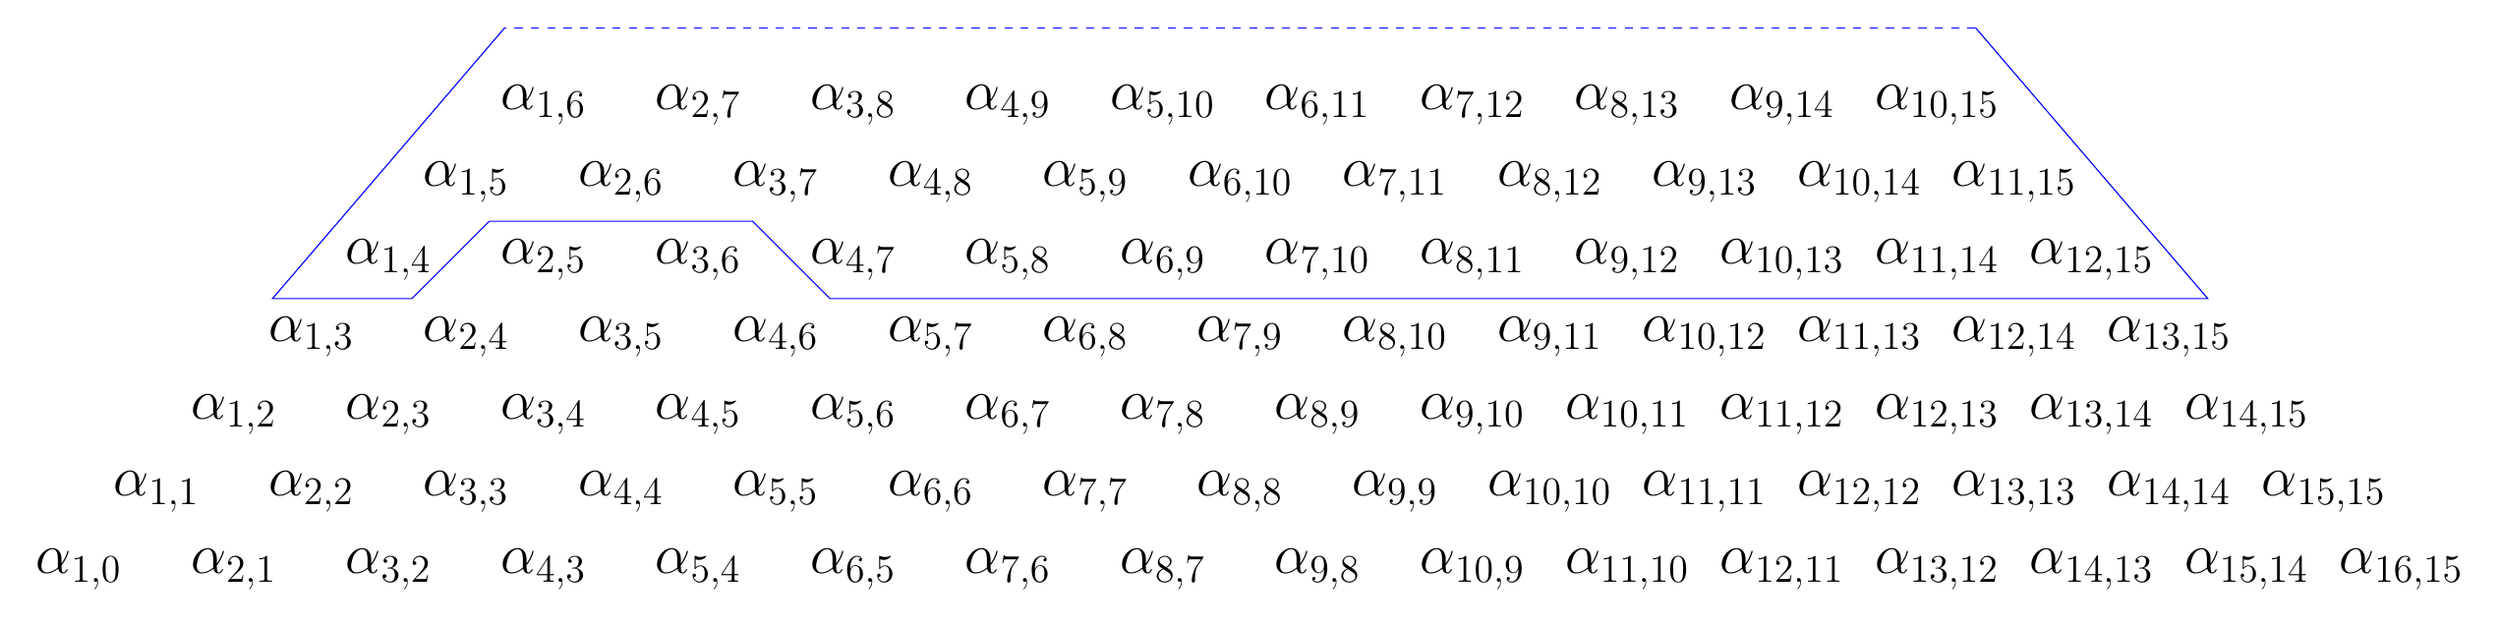
\begin{tikzpicture}[baseline={(0,-10)}]

\foreach \y in {9,...,15}
    \foreach \x in {0,..., \y }{
        \pgfmathsetmacro\cx{int(\x + 1)};
        \pgfmathsetmacro\cy{int(15 - \y + \x)};
        \pgfmathsetmacro\z{int(15 - \y - 1)};
        \ifthenelse{ \z > 2 }{ 
        \draw (-\y + 2*\x ,-\y) node {\huge $\alpha_{\cx,\cy}$};}{}
       }
\draw[blue] (-9.5,-8) -- (-12.5,-11.5) -- (-10.7,-11.5) -- (-9.7,-10.5) -- (-6.3,-10.5) -- (-5.3,-11.5) -- (12.5,-11.5) -- (9.5,-8);

\draw[dashed,blue] (9.5,-8) -- (-9.5,-8);

\end{tikzpicture}}

\def\excobktres{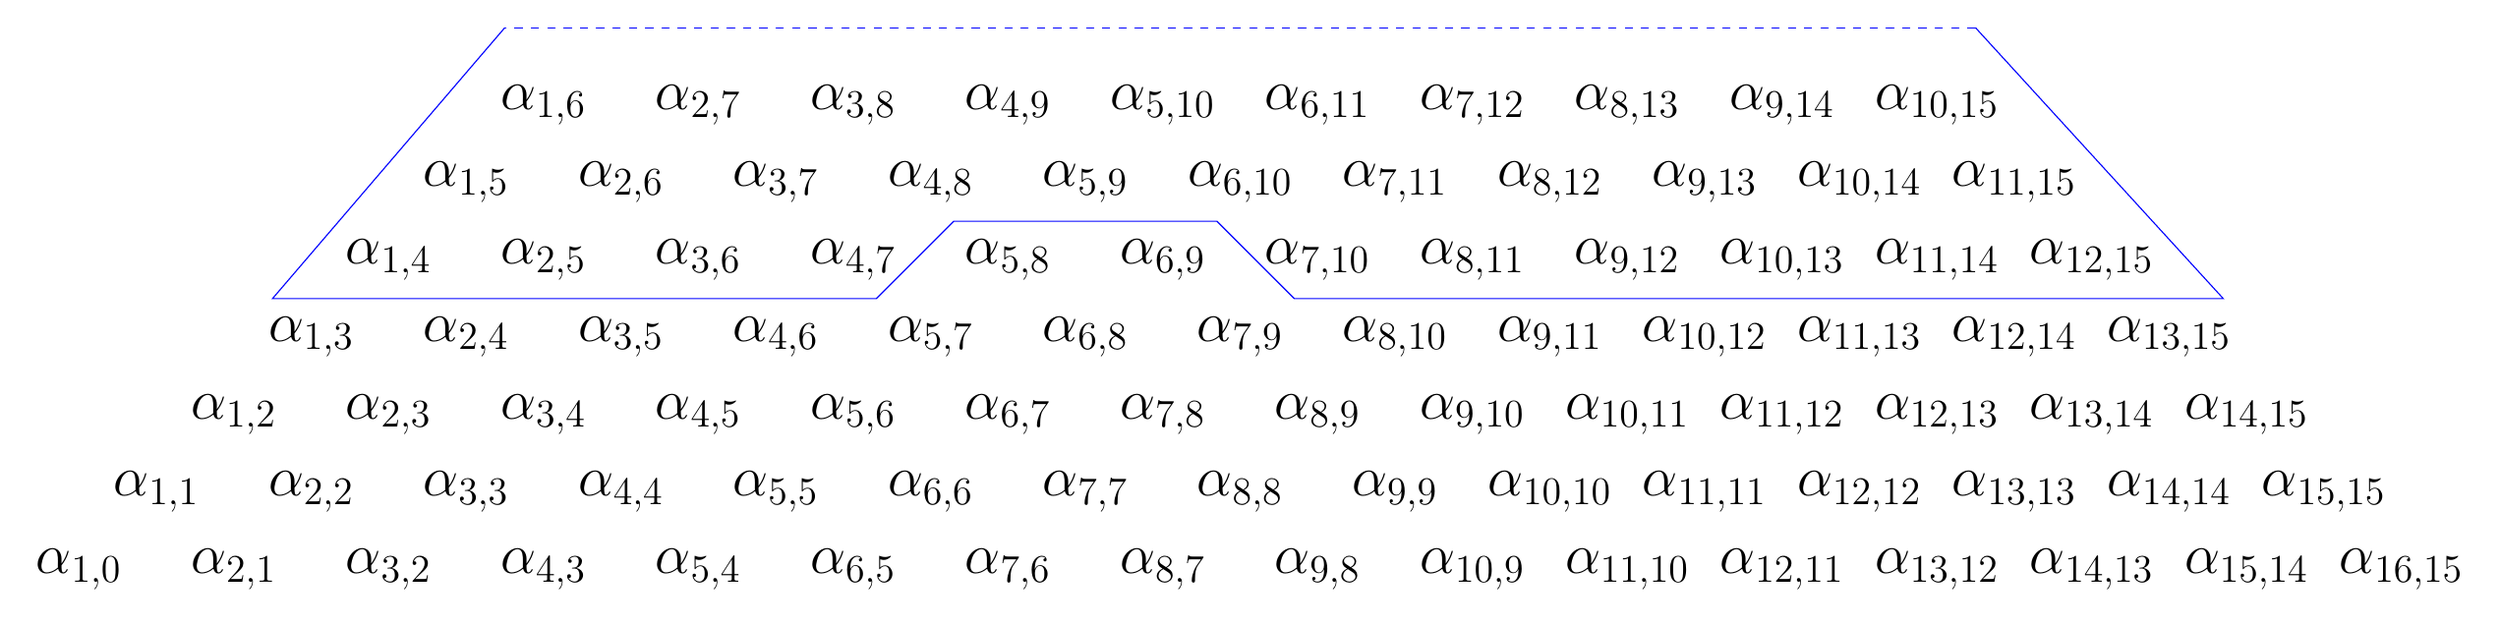
\begin{tikzpicture}[baseline={(0,-10)}]

\foreach \y in {9,...,15}
    \foreach \x in {0,..., \y }{
        \pgfmathsetmacro\cx{int(\x + 1)};
        \pgfmathsetmacro\cy{int(15 - \y + \x)};
        \pgfmathsetmacro\z{int(15 - \y - 1)};
        \ifthenelse{ \z > 2 }{ 
        \draw (-\y + 2*\x ,-\y) node {\huge $\alpha_{\cx,\cy}$};}{}
       }
\draw[blue] (-9.5,-8) -- (-12.5,-11.5) -- (-8.7,-11.5) --  (-5.3,-11.5) -- (-4.7,-11.5) -- (-3.7,-10.5) -- (-0.3,-10.5) -- (0.7,-11.5) -- (12.7,-11.5) -- (9.5,-8);

\draw[dashed,blue] (9.5,-8) -- (-9.5,-8);

\end{tikzpicture}}

\def\excobkcuatro{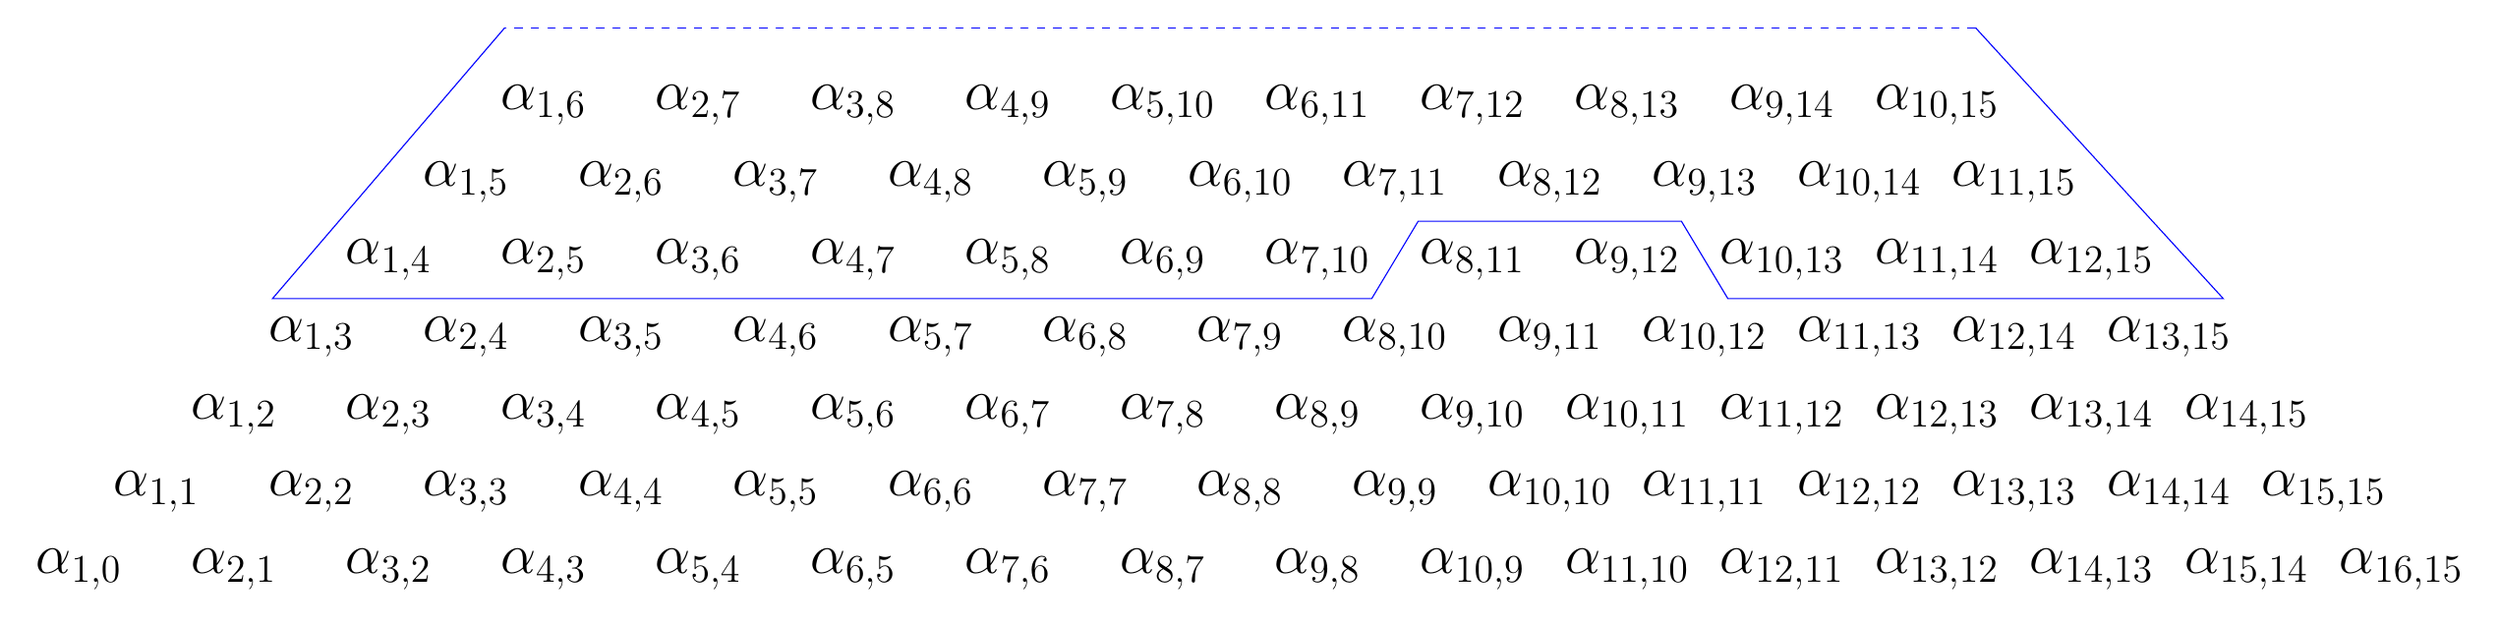
\begin{tikzpicture}[baseline={(0,-10)}]

\foreach \y in {9,...,15}
    \foreach \x in {0,..., \y }{
        \pgfmathsetmacro\cx{int(\x + 1)};
        \pgfmathsetmacro\cy{int(15 - \y + \x)};
        \pgfmathsetmacro\z{int(15 - \y - 1)};
        \ifthenelse{ \z > 2 }{ 
        \draw (-\y + 2*\x ,-\y) node {\huge $\alpha_{\cx,\cy}$};}{}
       }
\draw[blue] (-9.5,-8) -- (-12.5,-11.5) -- (-8.7,-11.5) --  (-5.3,-11.5) -- (-2.3,-11.5) -- (1.7,-11.5) -- (2.3,-10.5) -- (5.7,-10.5) -- (6.3,-11.5) -- (7.7,-11.5) -- (10.3,-11.5) --  (12.7,-11.5) -- (9.5,-8);

\draw[dashed,blue] (9.5,-8) -- (-9.5,-8);

\end{tikzpicture}}

\def\excobkcinco{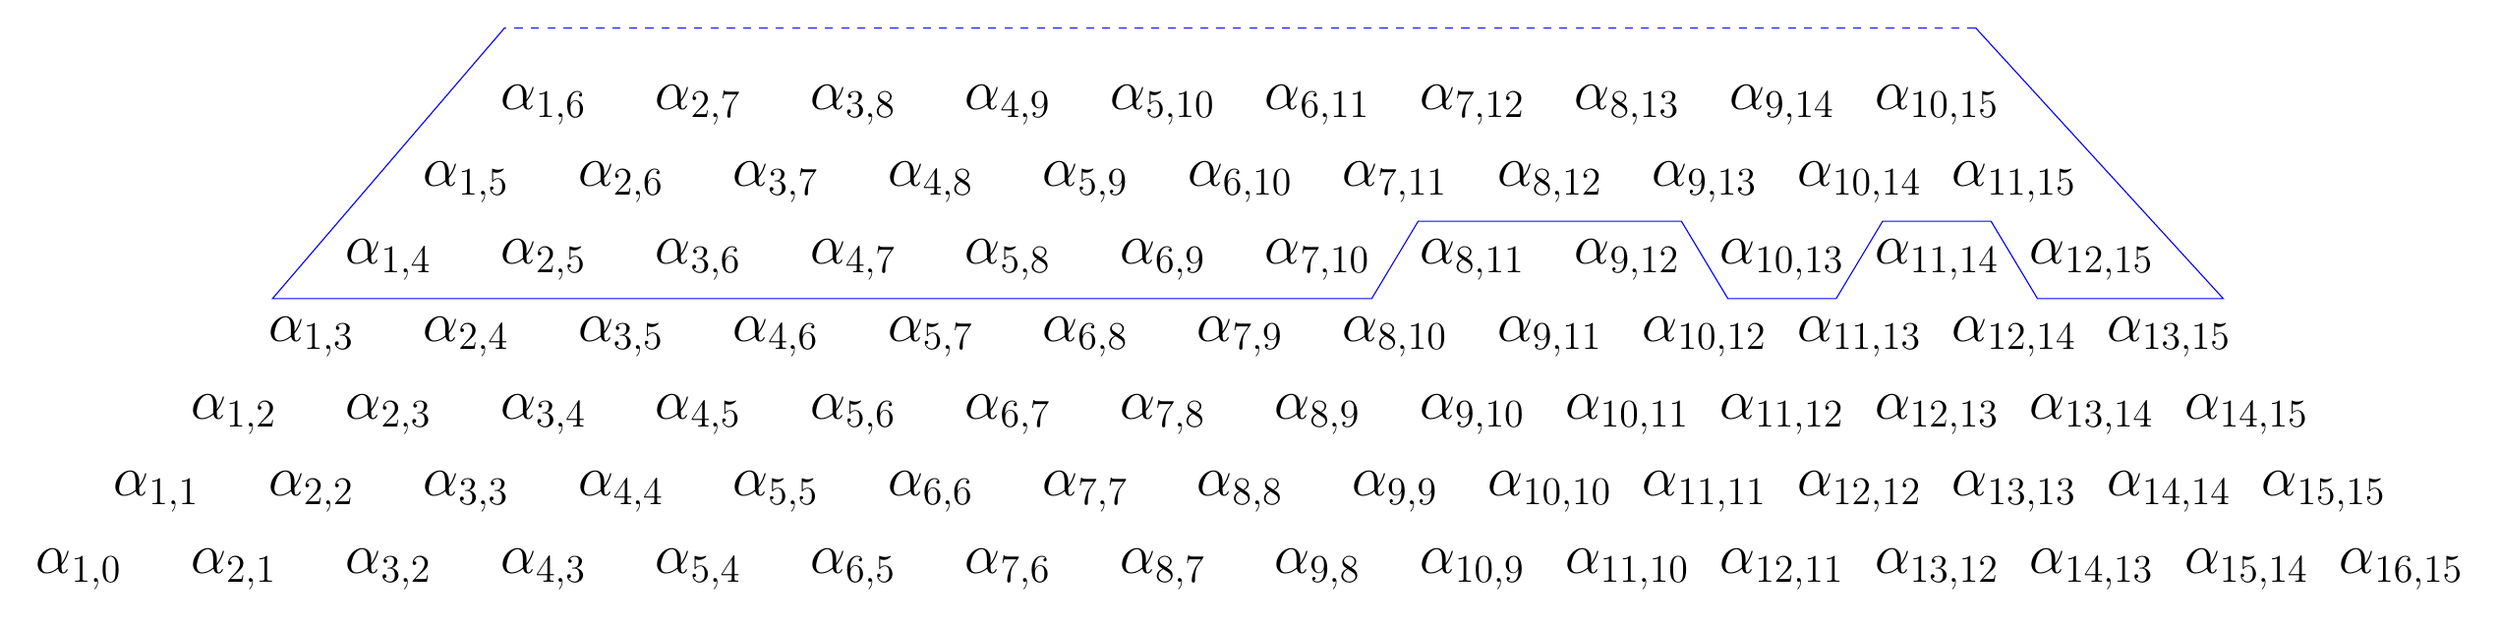
\begin{tikzpicture}[baseline={(0,-10)}]

\foreach \y in {9,...,15}
    \foreach \x in {0,..., \y }{
        \pgfmathsetmacro\cx{int(\x + 1)};
        \pgfmathsetmacro\cy{int(15 - \y + \x)};
        \pgfmathsetmacro\z{int(15 - \y - 1)};
        \ifthenelse{ \z > 2 }{ 
        \draw (-\y + 2*\x ,-\y) node {\huge $\alpha_{\cx,\cy}$};}{}
       }
\draw[blue] (-9.5,-8) -- (-12.5,-11.5) -- (-8.7,-11.5) --  (-5.3,-11.5) -- (-2.3,-11.5) -- (1.7,-11.5) -- (2.3,-10.5) -- (5.7,-10.5) -- (6.3,-11.5) -- (7.7,-11.5) -- (8.3,-10.5) -- (9.7,-10.5) -- (10.3,-11.5) --  (12.7,-11.5) -- (9.5,-8);

\draw[dashed,blue] (9.5,-8) -- (-9.5,-8);

\end{tikzpicture}}

\def\excobkseis{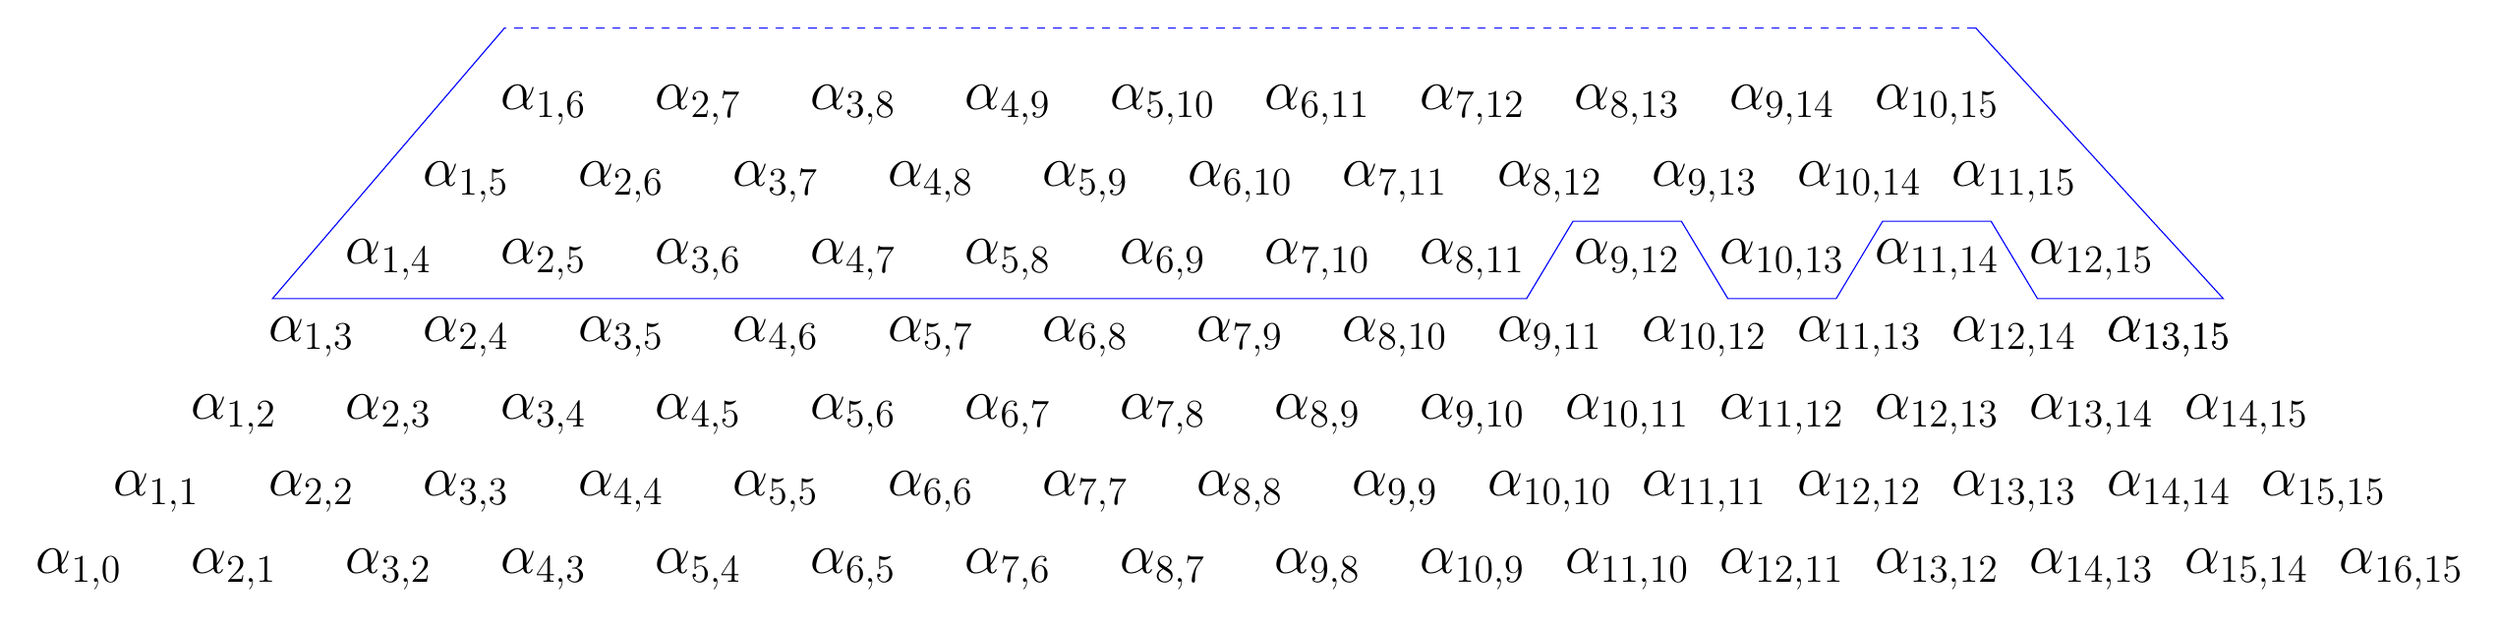
\begin{tikzpicture}[baseline={(0,-10)}]

\foreach \y in {9,...,15}
    \foreach \x in {0,..., \y }{
        \pgfmathsetmacro\cx{int(\x + 1)};
        \pgfmathsetmacro\cy{int(15 - \y + \x)};
        \pgfmathsetmacro\z{int(15 - \y - 1)};
        \ifthenelse{ \z > 2 }{ 
        \draw (-\y + 2*\x ,-\y) node {\huge $\alpha_{\cx,\cy}$};}{}
       }
\draw[blue] (-9.5,-8) -- (-12.5,-11.5) -- (-8.7,-11.5) --  (-5.3,-11.5) -- (3.7,-11.5) -- (4.3,-10.5) -- (5.7,-10.5) -- (6.3,-11.5) -- (7.7,-11.5) -- (8.3,-10.5) -- (9.7,-10.5) -- (10.3,-11.5) --  (12.7,-11.5) -- (9.5,-8);

\draw (12,-12) node {\huge $\alpha_{13,15}$};

\draw[dashed,blue] (9.5,-8) -- (-9.5,-8);

\end{tikzpicture}}



\def\exbonito{\begin{tikzpicture}[rotate=0]

  \foreach \y in {1,...,10}
    \foreach \x in {\y ,..., 10  }{
       \pic[fill=green!0] at (-1/2*\y +\x  ,\y) {square};
     }

 \foreach \y in {5,...,10}
    \foreach \x in {\y ,..., 10  }{
       \pic[fill=green!50] at (-1/2*\y +\x  ,\y) {square};
     }

 \foreach \x in {7,..., 10  }{
       \pic[fill=green!50] at (-1/2*4 +\x  ,4) {square};
     }
     
     \foreach \x in {1,..., 10 }{
\draw[] (\x ,1.5) node {\huge $\x$};
     }

\end{tikzpicture}}






\def\exbonitoB{\begin{tikzpicture}
  \foreach \y in {1,...,10}
    \foreach \x in {\y ,..., 10  }{
       \pic[fill=green!0] at (-1/2*\y +\x  ,\y) {square};
     }



 \foreach \x in {7,..., 9  }{
       \pic[fill=green!50] at (-1/2*4 +\x  ,4) {square};
     }

 \foreach \x in {8,..., 10  }{
       \pic[fill=green!50] at (-1/2*5 +\x  ,5) {square};
     }     

 \foreach \x in {9,..., 10  }{
       \pic[fill=green!50] at (-1/2*6 +\x  ,6) {square};
     }     

 \foreach \x in {10,..., 10  }{
       \pic[fill=green!50] at (-1/2*7 +\x  ,7) {square};
     }     

 \foreach \x in {5,..., 5  }{
       \pic[fill=green!50] at (-1/2*5 +\x  ,5) {square};
     }


 \foreach \x in {4,...,5  }{
       \pic[fill=red!50] at (-1/2*4 +\x  ,4) {square};
     }

 \foreach \x in {3,...,7  }{
       \pic[fill=red!50] at (-1/2*3 +\x  ,3) {square};
     }

 \foreach \x in {3,...,7  }{
       \pic[fill=red!50] at (-1/2*2 +\x  ,2) {square};
     }     
     
     \foreach \x in {1,..., 10 }{
\draw[] (\x ,1.5) node {\huge $\x$};
     }
     
     
\end{tikzpicture}}



\def\exbonitoC{\begin{tikzpicture}
  \foreach \y in {1,...,15}
    \foreach \x in {1,...,\y }{
       \pic[fill=green!50] at (15-\x,\y) {square};
     }
 \foreach \y in {1,...,15}{
       \pic[fill=red!50] at (15-\y,\y) {square};
     }
 \foreach \y in {2,...,15}{
       \pic[fill=red!50] at (16-\y,\y) {square};
     }     

 \foreach \y in {3,...,15}{
       \pic[fill=red!50] at (17-\y,\y) {square};
     } 

 \pic[fill=green!50] at (4,15) {square};
      
     
\end{tikzpicture}}

\def\lambdax{\ytableausetup{centertableaux}\ydiagram[*(cyan!30!)]{18,16,13,8,8,8,8,8,8,4,4,4,1}}

\def\lamdamenosseissiete{\ytableausetup{centertableaux}\ydiagram[*(cyan!30!)]{18,16,13,8,8,7,8,8,8,4,4,4,1}*[*(red!50!)]{0,0,0,0,0,7+1,0,0,0,0,0,0}*[*(blue!50!)]{0,0,0,0,0,0,0,0,8+1,0,0,0}}

\def\plambda{\ytableausetup{centertableaux}\ydiagram[*(cyan!30!)]{18,16,13,8,8,7,8,8,8,4,4,4,1}*[*(red!50!)]{0,0,0,0,0,7+1,0,0,0,0,0,0}*[*(blue!50!)]{0,0,0,0,0,0,0,0,8+1,0,0,0}}


\def\pplambda{\ytableausetup{centertableaux}\ydiagram[*(cyan!30!)]{18,16,12,8,7,8,8,8,8,4,4,4,1}*[*(red!50!)]{0,0,12+1,0,7+1,0,0,0,0,0,0,0}*[*(blue!50!)]{0,0,0,0,0,0,0,8+1,8+1,0,0,0}}

\def\vlamda{\ytableausetup{centertableaux}\ydiagram[*(cyan!30!)]{18,16,12,8,8,8,8,8,8,4,4,4,1}*[*(red!50!)]{0,0,12+1,0,0,0,0,0,0,0,0,0}*[*(blue!50!)]{0,0,0,0,0,0,0,0,0,0,0,0,1+1}}

\def\pvlamda{\ytableausetup{centertableaux}\ydiagram[*(cyan!30!)]{18,16,12,8,7,8,8,8,8,4,4,4,1}*[*(red!50!)]{0,0,12+1,0,7+1,0,0,0,0,0,0,0}*[*(blue!50!)]{0,0,0,0,0,0,0,8+1,0,0,0,0,1+1}}

\def\ppplamda{\ytableausetup{centertableaux}\ydiagram[*(cyan!30!)]{18,15,12,7,8,8,8,8,8,4,4,4,1}*[*(red!50!)]{0,15+1,12+1,7+1,0,0,0,0,0,0,0,0}*[*(blue!50!)]{0,0,0,0,0,0,8+1,8+1,8+1,0,0,0}}

\def\vdoslamda{\ytableausetup{centertableaux}\ydiagram[*(cyan!30!)]{18,15,12,8,8,8,8,8,8,4,4,4,1}*[*(red!50!)]{0,15+1,12+1,0,0,0,0,0,0,0,0,0}*[*(blue!50!)]{0,0,0,0,0,0,0,0,0,4+1,0,0,1+1}}

\def\pvdoslamda{\ytableausetup{centertableaux}\ydiagram[*(cyan!30!)]{18,15,12,7,8,8,8,8,8,4,4,4,1}*[*(red!50!)]{,15+1,12+1,7+1,0,0,0,0,0,0,0,0}*[*(blue!50!)]{0,0,0,0,0,0,8+1,0,0,4+1,0,0,1+1}}

\def\vvlamda{\ytableausetup{centertableaux}\ydiagram[*(cyan!30!)]{18,15,12,8,8,8,8,8,8,4,4,4,1}*[*(red!50!)]{0,15+1,12+1,0,0,0,0,0,0,0,0,0}*[*(blue!50!)]{0,0,0,0,0,0,0,0,0,4+1,4+1}}

\def\pvvlamda{\ytableausetup{centertableaux}\ydiagram[*(cyan!30!)]{17,15,12,8,8,8,8,8,8,4,4,4,1}*[*(red!50!)]{17+1,15+1,12+1,0,0,0,0,0,0,0,0,0}*[*(blue!50!)]{0,0,0,0,0,0,8+1,0,0,4+1,4+1}}
 
\def\ppvlamda{\ytableausetup{centertableaux}\ydiagram[*(cyan!30!)]{17,15,12,8,8,8,8,8,8,4,4,4,1}*[*(red!50!)]{17+1,15+1,12+1,0,0,0,0,0,0,0,0,0}*[*(blue!50!)]{0,0,0,0,0,0,8+1,8+1,0,0,0,0,1+1}}

\def\dibujitoprueba{\scalebox{0.3}{\ytableausetup{centertableaux}\ydiagram[*(cyan!30!)]{17,15,12,8,8,8,8,8,8,4,1}*[*(red!50!)]{17+1,15+1,12+1,0,0,0,0,0,0,0,0,0}*[*(blue!50!)]{0,0,0,0,0,0,8+1,0,0,4+1,0,0,1+1}}}


\def\pppplamda{\ydiagram[*(cyan!30!)]{16,14,11,8,8,8,8,8,8,4,4,4,1}*[*(red!50!)]{16+2,14+2,11+2,0,0,0,0,0,0,0,0,0}*[*(blue!50!)]{0,0,0,8+1,8+1,8+1,8+1,8+1,8+1,0,0,0}}

\def\ppvdoslamda{\ydiagram[*(cyan!30!)]{16,14,11,8,8,8,8,8,8,4,4,4,1}*[*(red!50!)]{16+2,14+2,11+2,0,0,0,0,0,0,0,0,0}*[*(blue!50!)]{0,0,0,8+1,8+1,8+1,8+1,0,0,4+1,0,0,1+1}}

\def\ppvvlamda{\ydiagram[*(cyan!30!)]{16,14,11,8,8,8,8,8,8,4,4,4,1}*[*(red!50!)]{16+2,14+2,11+2,0,0,0,0,0,0,0,0,0}*[*(blue!50!)]{0,0,0,8+1,8+1,8+1,8+1,0,0,4+1,4+1}}

\def\pppvlamda{\ydiagram[*(cyan!30!)]{16,14,11,8,8,8,8,8,8,4,4,4,1}*[*(red!50!)]{16+2,14+2,11+2,0,0,0,0,0,0,0,0,0}*[*(blue!50!)]{0,0,0,8+1,8+1,8+1,8+1,8+1,0,0,0,0,1+1}}

\def\grandiagramados{\begin{tikzpicture}
    \node at (-2.5,3) (k) {\scalebox{0.25}{\lambdax}};
    \node[draw] at (-4.5,0) (l) {\scalebox{0.25}{\lambdax}};
    
    \node at (0,0) (a) {\scalebox{0.25}{\plambda}};
    
    \node at (-4,-3) (b) {\scalebox{0.25}{\pplambda}};
    \node[draw] at (0,-3) (c) {\scalebox{0.25}{\vlamda}};
    \node[draw] at (4,-3) (d) {\scalebox{0.25}{\pvlamda}};

    \node[draw] at (-7.5,-6) (b1) {\scalebox{0.25}{\ppplamda}};
    \node[draw] at (-4.5,-6) (b2) {\scalebox{0.25}{\vvlamda}};
    \node[draw] at (-1.5,-6) (b3) {\scalebox{0.25}{\pvvlamda}};

    % \node at (1.5,-6) (d1) {\scalebox{0.3}{\ppvlamda}};
    % \node at (4.5,-6) (d2) {\scalebox{0.3}{\vdoslamda}};
    % \node at (7.5,-6) (d3) {\scalebox{0.3}{\pvdoslamda}};

    % \node[draw] at (-7.5,-9) (b11) {\scalebox{0.25}{\pppplamda}};
    % \node at (-1.5,-9) (b33) {\scalebox{0.3}{\ppvvlamda}};

    % \node at (1.5,-9) (d11) {\scalebox{0.3}{\pppvlamda}};
    % \node at (7.5,-9) (d33) {\scalebox{0.3}{\ppvdoslamda}};
    
    \draw[->] (k.south) -- node[above] {$-q$} (a.north);
    \draw[->] (k.south) -- node[left] {$1$} (l.north);
    
    \draw[->] (a.south) -- node[above] {$q^2$} (b.north);
    \draw[->] (a.south) -- node[left] {$q^5$} (c.north);
    \draw[->] (a.south) -- node[above] {$-q^6$} (d.north);

    \draw[->] (b.south) -- node[above] {$q^2$} (b1.north);
    \draw[->] (b.south) -- node[left] {$q^5$} (b2.north);
    \draw[->] (b.south) -- node[above] {$-q^6$} (b3.north);

    % \draw[->] (d.south) -- node[above] {$q^2$} (d1.north);
    % \draw[->] (d.south) -- node[left] {$q$} (d2.north);
    % \draw[->] (d.south) -- node[above] {$-q^3$} (d3.north);

    % \draw[->] (b1.south) -- node[left] {$q^3$} (b11.north);
    % \draw[->] (b3.south) -- node[left] {$q^3$} (b33.north);

    % \draw[->] (d1.south) -- node[left] {$q^3$} (d11.north);
    % \draw[->] (d3.south) -- node[left] {$q^3$} (d33.north);
\end{tikzpicture}}




%%%%%%%%%%%%%%%%%%%%%%%%%%%%%%%%%%%%

\def\exLemmaBKA{\begin{tikzpicture}[rotate=0]

  \foreach \y in {1,...,10}
    \foreach \x in {\y ,..., 10  }{
       \pic[fill=green!0] at (-1/2*\y +\x  ,\y) {square};
     }

 \foreach \y in {5,...,10}
    \foreach \x in {\y ,..., 10  }{
       \pic[fill=green!50] at (-1/2*\y +\x  ,\y) {square};
     }

 \foreach \x in {8,..., 10  }{
       \pic[fill=green!50] at (-1/2*4 +\x  ,4) {square};
     }
     
     \foreach \x in {1,..., 10 }{
\draw[] (\x ,1.5) node {\huge $\x$};
     }

 \foreach \x in {4,...,4  }{
       \pic[fill=green!50] at (-1/2*4 +\x  ,4) {square};
     }     

\end{tikzpicture}}
      


\def\exLemmaBKB{\begin{tikzpicture}[rotate=0]

  \foreach \y in {1,...,10}
    \foreach \x in {\y ,..., 10  }{
       \pic[fill=green!0] at (-1/2*\y +\x  ,\y) {square};
     }

 \foreach \y in {5,...,10}
    \foreach \x in {\y ,..., 10  }{
       \pic[fill=green!50] at (-1/2*\y +\x  ,\y) {square};
     }

 \foreach \x in {9,..., 10  }{
       \pic[fill=green!50] at (-1/2*4 +\x  ,4) {square};
     }
     
     \foreach \x in {1,..., 10 }{
\draw[] (\x ,1.5) node {\huge $\x$};
     }

 \foreach \x in {4,...,5  }{
       \pic[fill=green!50] at (-1/2*4 +\x  ,4) {square};
     }     

\end{tikzpicture}}





\def\exLemmaBKC{\begin{tikzpicture}[rotate=0]

  \foreach \y in {1,...,10}
    \foreach \x in {\y ,..., 10  }{
       \pic[fill=green!0] at (-1/2*\y +\x  ,\y) {square};
     }

 \foreach \y in {5,...,10}
    \foreach \x in {\y ,..., 10  }{
       \pic[fill=green!50] at (-1/2*\y +\x  ,\y) {square};
     }

 \foreach \x in {10,..., 10  }{
       \pic[fill=green!50] at (-1/2*4 +\x  ,4) {square};
     }
     
     \foreach \x in {1,..., 10 }{
\draw[] (\x ,1.5) node {\huge $\x$};
     }

 \foreach \x in {4,...,6  }{
       \pic[fill=green!50] at (-1/2*4 +\x  ,4) {square};
     }     

\end{tikzpicture}}


\def\exLemmaBKD{\begin{tikzpicture}[rotate=0]

  \foreach \y in {1,...,10}
    \foreach \x in {\y ,..., 10  }{
       \pic[fill=green!0] at (-1/2*\y +\x  ,\y) {square};
     }

 \foreach \y in {5,...,10}
    \foreach \x in {\y ,..., 10  }{
       \pic[fill=green!50] at (-1/2*\y +\x  ,\y) {square};
     }

 % \foreach \x in {10,..., 10  }{
 %       \pic[fill=green!50] at (-1/2*4 +\x  ,4) {square};
 %     }
     
     \foreach \x in {1,..., 10 }{
\draw[] (\x ,1.5) node {\huge $\x$};
     }

 \foreach \x in {4,...,7  }{
       \pic[fill=green!50] at (-1/2*4 +\x  ,4) {square};
     }     

\end{tikzpicture}}

\newcommand{\dibu}[3]{
\pgfmathsetmacro\cx{int(#3) -int(#2) + 2};
\pgfmathsetmacro\cxu{int(\cx)-1};
\pgfmathsetmacro\cxd{int(#3)+ 1};
  \foreach \y in {1,...,#1}
    \foreach \x in {\y ,..., #1  }{
       \pic[fill=green!0] at (-1/2*\y +\x  ,\y) {square};
     }

 \foreach \y in {\cx,...,#1}
    \foreach \x in {\y ,..., #1  }{
       \pic[fill=green!50] at (-1/2*\y +\x  ,\y) {square};
     }

 \foreach \x in {\cxd,..., #1  }{
       \pic[fill=green!50] at (-1/2*\cxu  +\x  ,\cxu) {square};
     }
     
     \foreach \x in {1,..., #1 }{
\draw[] (\x ,1.5) node {\huge $\x$};
     }}

\newcommand{\dibuB}[3]{
\pgfmathsetmacro\cx{int(#3) -int(#2) + 2};
\pgfmathsetmacro\cxu{int(\cx)-1};
\pgfmathsetmacro\cxd{int(#3)+ 1};
  \foreach \y in {1,...,#1}
    \foreach \x in {\y ,..., #1  }{
       \pic[fill=green!0] at (-1/2*\y +\x  ,\y) {square};
     }

 \foreach \y in {\cx,...,#1}
    \foreach \x in {\y ,..., #1  }{
       \pic[fill=green!0] at (-1/2*\y +\x  ,\y) {square};
     }

 \foreach \x in {\cxd,..., #1  }{
       \pic[fill=green!0] at (-1/2*\cxu  +\x  ,\cxu) {square};
     }
     
     \foreach \x in {1,..., #1 }{
\draw[] (\x ,1.5) node {\huge $\x$};
     }}

\newcommand{\agregof}[3]{
\pgfmathsetmacro\altx{int(#1)};
 \foreach \x in {#2,..., #3  }{
       \pic[fill=green!50] at (1/2*\altx  +\x-1  ,\altx) {square};
     }
}

\newcommand{\quitof}[3]{
\pgfmathsetmacro\altx{int(#1)};
 \foreach \x in {#2,..., #3  }{
       \pic[fill=white] at (1/2*\altx  +\x-1  ,\altx) {square};
     }
}

\newcommand{\quitoS}[3]{
\pgfmathsetmacro\altx{int(#1)};
\pgfmathsetmacro\xx{int(#2)};
 \foreach \x in {0,..., #3  }{
       \pic[fill=red] at (1/2*\altx  +\xx-1 -1/2*\x,\altx +\x) {square};
     }
}
\newcommand{\agregoA}[3]{
\pgfmathsetmacro\altx{int(#1)};
\pgfmathsetmacro\xx{int(#2)};
 \foreach \x in {0,..., #3  }{
       \pic[line width=4pt] at (1/2*\altx  +\xx-1 +1/2*\x,\altx +\x) {square};
     }
}

\newcommand{\agregoR}[3]{
\pgfmathsetmacro\altx{int(#1)};
 \foreach \x in {#2,..., #3  }{
       \pic[fill=red] at (1/2*\altx  +\x-1  ,\altx) {square};
     }
}

\newcommand{\peso}[9]{
 \foreach \x / \y in {1/1,2/0,3/0,4/0,5/0,6/0,7/0,8/#1,9/#2,10/#3,11/#4,12/#5,13/#6,14/#7,15/#8,16/#9}{
       \draw[] (\x ,0.5) node {\huge $\y$ };
     }
}

\newcommand{\pesoTrap}[3]{
 \foreach \x / \y in {1/1,2/2,3/3,4/4,5/5,6/0,7/0,8/#1,9/#2,10/10,11/11,12/12,13/#3}{
       \draw[] (\x ,0.5) node {\huge $\y$ };
     }
}